\documentclass{mcmthesis}
\mcmsetup{CTeX = true,    % 使用 CTeX 套装时,设置为 true
          tcn = \textcolor{black}{2202009}, problem = {A},
          sheet = true, titleinsheet = true, keywordsinsheet = true,
          titlepage = false, abstract = false}
\usepackage{array}       
\usepackage{newtxtext}     % \usepackage{palatino}
\usepackage[backend=bibtex]{biblatex}   % for RStudio Complie
\usepackage{lipsum}
\usepackage{wrapfig}
\usepackage{fancyhdr}
\fancypagestyle{plain}

\title{Power-Time-Energy Model in Cycling}
% \author{\small \href{http://www.latexstudio.net/}
%   {
\includegraphics[width=7cm]{mcmthesis-logo}}}
\date{\today}

\begin{document}

\begin{abstract}
\par Despite differences between types of races, minimizing the time to cover a certain course has always been the core of cycling. In our paper, Power-Time-Energy (PTE) Model is established, including three sub-models: Power Curve Fitting, Power-Time-Energy (PTE) Equation and Optimizer. PTE model analyzes the relationship between various affecting factors during cycling and rider's optimal power output.

\par Firstly, power profiles of cyclists from world-class to fair level are collected, defined as the maximum duration a rider can hold on at different exercise intensity. Based on power profiles, different cyclists' power curves are well fitted, including time trialists and sprinters of different genders. Values of adjusted $R^2$ up to 0.98 indicate the goodness of the fit.

\par Then, PTE Equation is constructed to bridge the power output and energy required in competition process based on the power profile and rider's position on the track(length and elevation gain). We next use Optimizer to produce strategy which is separated into three stages: FTP-Recovery-Sprint. To verify the rationality, we make simulation: two world-class virtual time trialists are created to participate in Olympics ITT, UCI WCTT and one self-designed race, adopting tactics provided by PTE Model. It turns out that our virtual riders rank high in these games after comparing with the real result data.

\par Next, we conduct sensitivity analysis with respect to weather conditions (wind direction and speed) and get positive feedback. Under the framework of PTE model, we put forward and prove Wind Direction Theorem. It indicates that constant direction has no effect on the total energy cost of a closed track, and in non-closed cases, the effect is only related to the location of start and end points. Moreover, optimal tactics will change appropriately according to different wind speed in our simulation.

\par Besides, the model simulates different power output at each stage and provides optimal tactics separately. The result indicates that change in total time is minor as the output power deviates to some degree. Considering the difficulty for riders to execute strategies accurately, this property ensures that the cyclist can still achieve satisfactory results under the condition of deviation.

\par Finally, our model has strong extensibility: it can also be applied to team time trial consisting of 6 riders. The whole process is divided into three stages, with 6, 5 and 4 riders uniting the team respectively. In our basic strategy, riders take turns to block the wind to keep high constant speed and the four most energetic riders will reach the end together. Similar to PTE Model, we set up corresponding equations and constraints for each stage, together with an optimization model that customizes the best tactic for a team.

 
\begin{keywords}
Time Trial, Power Distribution, Nonlinear Optimization,  MATLAB
\end{keywords}

\end{abstract}

\maketitle

%% Generate the Table of Contents, if it's needed.
\tableofcontents   % 若不想要目录, 注释掉该句

\newpage


\section{Introduction}

\subsection{Problem background}
\par Cyclists are divided into different categories, such as sprinters, persuiters, time trivalists, and so on. Different types of riders may have different power curves. The power curve depicts how long an athlete can sustain a given power output, which can help cyclists plan their energy more wisely during the competition.
\par There are many types of cycling competitions, but the common denominator is that all cyclists complete the same distance in less time than anyone else. Therefore cyclists are always looking for how to complete a given distance in less time, and how to develop training plans and competition strategies through the power curve becomes increasingly important.


\subsection{Restatement of the Problem}
\par Build a mathematical model that describes the relationship between a cyclist's position and the energy released, which can be applied to different types of riders. The model must take into account the constraints on the total energy released by the cyclist, and the limits of both past overloading and the power curve.
\begin{itemize}
	\item {\bf The first problem requires to describe power profiles of two types of cyclists}, one of which is a time trial specialist, and consider different genders.
	\item {\bf The second problem talks about the application of the model in various time trial races}, including 2021 Olympic Time Trial course, 2021 UCI World Championship time trial course and a self-designed course with at least four sharp turns and a nontrivial road grade.
	\item {\bf The third problem argues the potential impact of different environmental conditions.} It demands us to test the sensitivity of the model.
	\item {\bf The fourth problem focuses on cyclists' imperfectly execution on power distribution.} It asks to provide a detailed plan for riders.
	\item {\bf The fifth problem discusses the extension of the model.} The aim is to produce the best distribution of energy for teams of six in a team time trival.
\end{itemize}


\subsection{Our work}
In a gesture to plot the power profile, propose the optimal riding strategy and test the sensitivity of the model, several works are done to build it and then solve the problem.
\begin{itemize}
	\item{\bf Accessing the data}. As it's hard to get real-time speed data of a certain athlete in a formal competition, we changed our course to excavate data from standard pace, past papers and other resources.The data sources are summarized in table [\ref{data}].
		\begin{table}[htbp]
				%	\renewcommand\arraystretch{1.3}
		%	\setlength\tabcolsep{13pt}%调列距
			\setlength{\belowcaptionskip}{0.2cm}
		\centering
		\caption{Data Source Collection}
		\begin{tabular}{cc}
			\toprule[2pt]
			Dataset & Website Source \\
			\midrule
			Cycling power charts & \textcolor[rgb]{ .02,  .388,  .757}{https://www.trainingpeaks.com/blog/power-profiling/} \\
			UCI results & \textcolor[rgb]{ .02,  .388,  .757}{https://www.flanders2021.com/en/races} \\
			Olympics results & \textcolor[rgb]{ .02,  .388,  .757}{https://www.procyclingstats.com/race/olympic-games-itt/2021/result} \\
			Maps  & \textcolor[rgb]{ .02,  .388,  .757}{https://www.openstreetmap.org/about/} \\
			Cycling details & \textcolor[rgb]{ .02,  .388,  .757}{https://www.strava.com/activities} \\
			\bottomrule[2pt]
		\end{tabular}%
		\label{data}%
	\end{table}%
	\item {\bf Presenting our model}. In order to investigate the problem deeper, we divide our model into three sub-models. The first one is the establishment of \emph{Power Curve Fitting} to describe athletes' ability in different exercise intensity. The second one is about power distribution during competition process, \emph{Power-Time-Energy Equation}, which establishes the relationship between output energy and demand energy. The third one is to solve the optimal strategy for a certain player and certain competition.
	
	% TODO: \usepackage{graphicx} required
	\begin{figure}
		\centering
		
\includegraphics[width=0.7\linewidth]{image/liucheng}
		\caption{Structure chart}
		\label{liucheng}
	\end{figure}
	
	\item {\bf Sensitivity analysis and extension}.Taking weather condition and rider deviations into account, we apply extended model with UCI data to evaluate the reliability of our model through sensitivity analysis. Also, we extend our model to team time trial. 
	
\end{itemize}

\section{Assumptions and Justification}
To simplify the problem and make it convenient for us to simulate real-life conditions, we make the following basic assumptions, each of which is properly justified.

\begin{itemize}
	\item {\bf The rider has a limit on total energy}.  Considering real-life conditions, it is reasonable and necessary to assume that a rider has a limited total energy.
	
	\item {\bf The rider's total energy and power curve are invariable}. To simplify the model, we assume that the rider's total energy is unchangable regardless of weather, track and other things.
	
	\item {\bf The energy needed to finish a competition is proportionate to the athlete's weight}. To simplify the model, we consider that the energy needed to finish the same course for different athletes of the same weight is unchangeable and the needed power is only associated with weight.
	
	\item{\bf The competition record of an athlete is divided into several uniform motions.} Though the speed of the rider is real-time changing, it is reasonale to simulate the process by dividing the whole time into several parts and calculate the average speed separately. 
	
	\item{\bf Wind direction and speed remain the same during a race.} In our analysis, race times usually last around an hour, so the changes in wind conditions tend to be small.
	
\end{itemize}
\newpage
\section{Notations and Glossary}
\begin{center}
	%\renewcommand\arraystretch{1.3}
	%\setlength\tabcolsep{20pt}%调列距
	\begin{tabular}{p{1.5cm}<{\centering}p{11.5cm}<{\centering}p{2.5cm}<{\centering}}
		\toprule[2pt]
		{\bf Symbols} & {\bf Description} & \quad {\bf Unit} \\\midrule[1pt]
		$PO$ & power output of an athlete per kilogram  & \quad W/kg 
		\\[0.2cm]
		$t$ & maximum duration that a rider can maintain a certain speed  & \quad s \\[0.2cm]
	%	$CP$ & critical power per kilogram that divide heavy,moderate intensity domain and severe, extreme intensity domain & \quad W/kg \\[0.2cm]
		$T_i$ & the interval length of the $i^{th}$ time period &\quad s\\ [0.2cm]
		$P_i$ & average power per kilogram of the $i^{th}$ time period & \quad W/kg \\[0.2cm]
		$W_i$& work capacity one can expend of the $i^{th}$ time period & \quad km\\[0.2cm]
        $\sigma$& symbol for track model & \quad /\\
       	$E(s)$& the energy consumed per kilometer per kilogram at the position of s& \quad J/(kg$\cdot$km)\\[0.2cm]
		$\bar{E}$ &the energy consumed per kilometer per kilogram under the windless condition of a flat ground  & \quad J/(kg$\cdot$km)\\[0.2cm]
		
        $v$ & the speed of wind & \quad m/s\\[0.2cm]
        
        $\theta(s)$ &the angle between rider's forward direction and wind at the position of s & \quad /\\[0.2cm]
        $\phi(s)$& the slope gradient at the position of s&\quad /\\[0.2cm]
	\bottomrule[2pt]\\
	\end{tabular}
\end{center}
\noindent where we define the main parameters while specific value of those parameters will be given later.

\par We also give out the explanation of some proper nouns:
\begin{itemize}
	\item {\bf Functional threshold power (FTP) } Maximum mean power that a cyclist can sustainably produce for the period of one hour which can be expressed in terms of watts per kilo.
	\item {\bf Power Profile Chart} It shows how does rider's maximum power output compare to the riders of various fitness and experience level, ranging from novice to the world-class, pro road cyclists.The chart includes 4 values divided by weight reflecting one's cycling talent: sprint abilities (5s), anaerobic capacity described by 1 minute maximum power, 5 minutes to tell about maximum oxygen uptake capability and 20 min to describe FTP. 
	\item{\bf Power Curve} Optimal average power output from 1 second to maximum riding time measured in watts (W) or watts per kilogram (W/kg).

	\item {\bf W} Work capacity one can expend above the FTP before reaching complete exhaustion. 
	%In our model, we assume that CP equals FTP.
	\item{\bf Time Trialist(TT)} A road bicycle racer who can maintain high speeds for long periods of time, to maximize performance during individual or team time trials. 
	\item{\bf Sprinter} A road bicycle racer or track racer who can finish a race very explosively by accelerating quickly to a high speed.
	\item{\bf Hors catégorie (HC)} It is  the most difficult type of climb in a race. The average HC climb is 15-20 kilometers long and has a grade of 9\% while the easiest category of a climb is called Category 4 with elevation gain of less than 300 meters.
\end{itemize}

\section{Solution of the First Problem}
\begin{flushleft}
\qquad As we all know, the amount of time a person can maintain high-intensity exercise is often limited, so we use power curve to describe the relationship between power output and the longest time one man can maintain output of this level. Obviously, power curve differs from person to person, and there is a significant difference between both genders and rider types, such as climber, puncheur and time trial specialist. 
\end{flushleft}
\begin{wrapfigure}{l}{11cm} % 靠文字内容的左侧
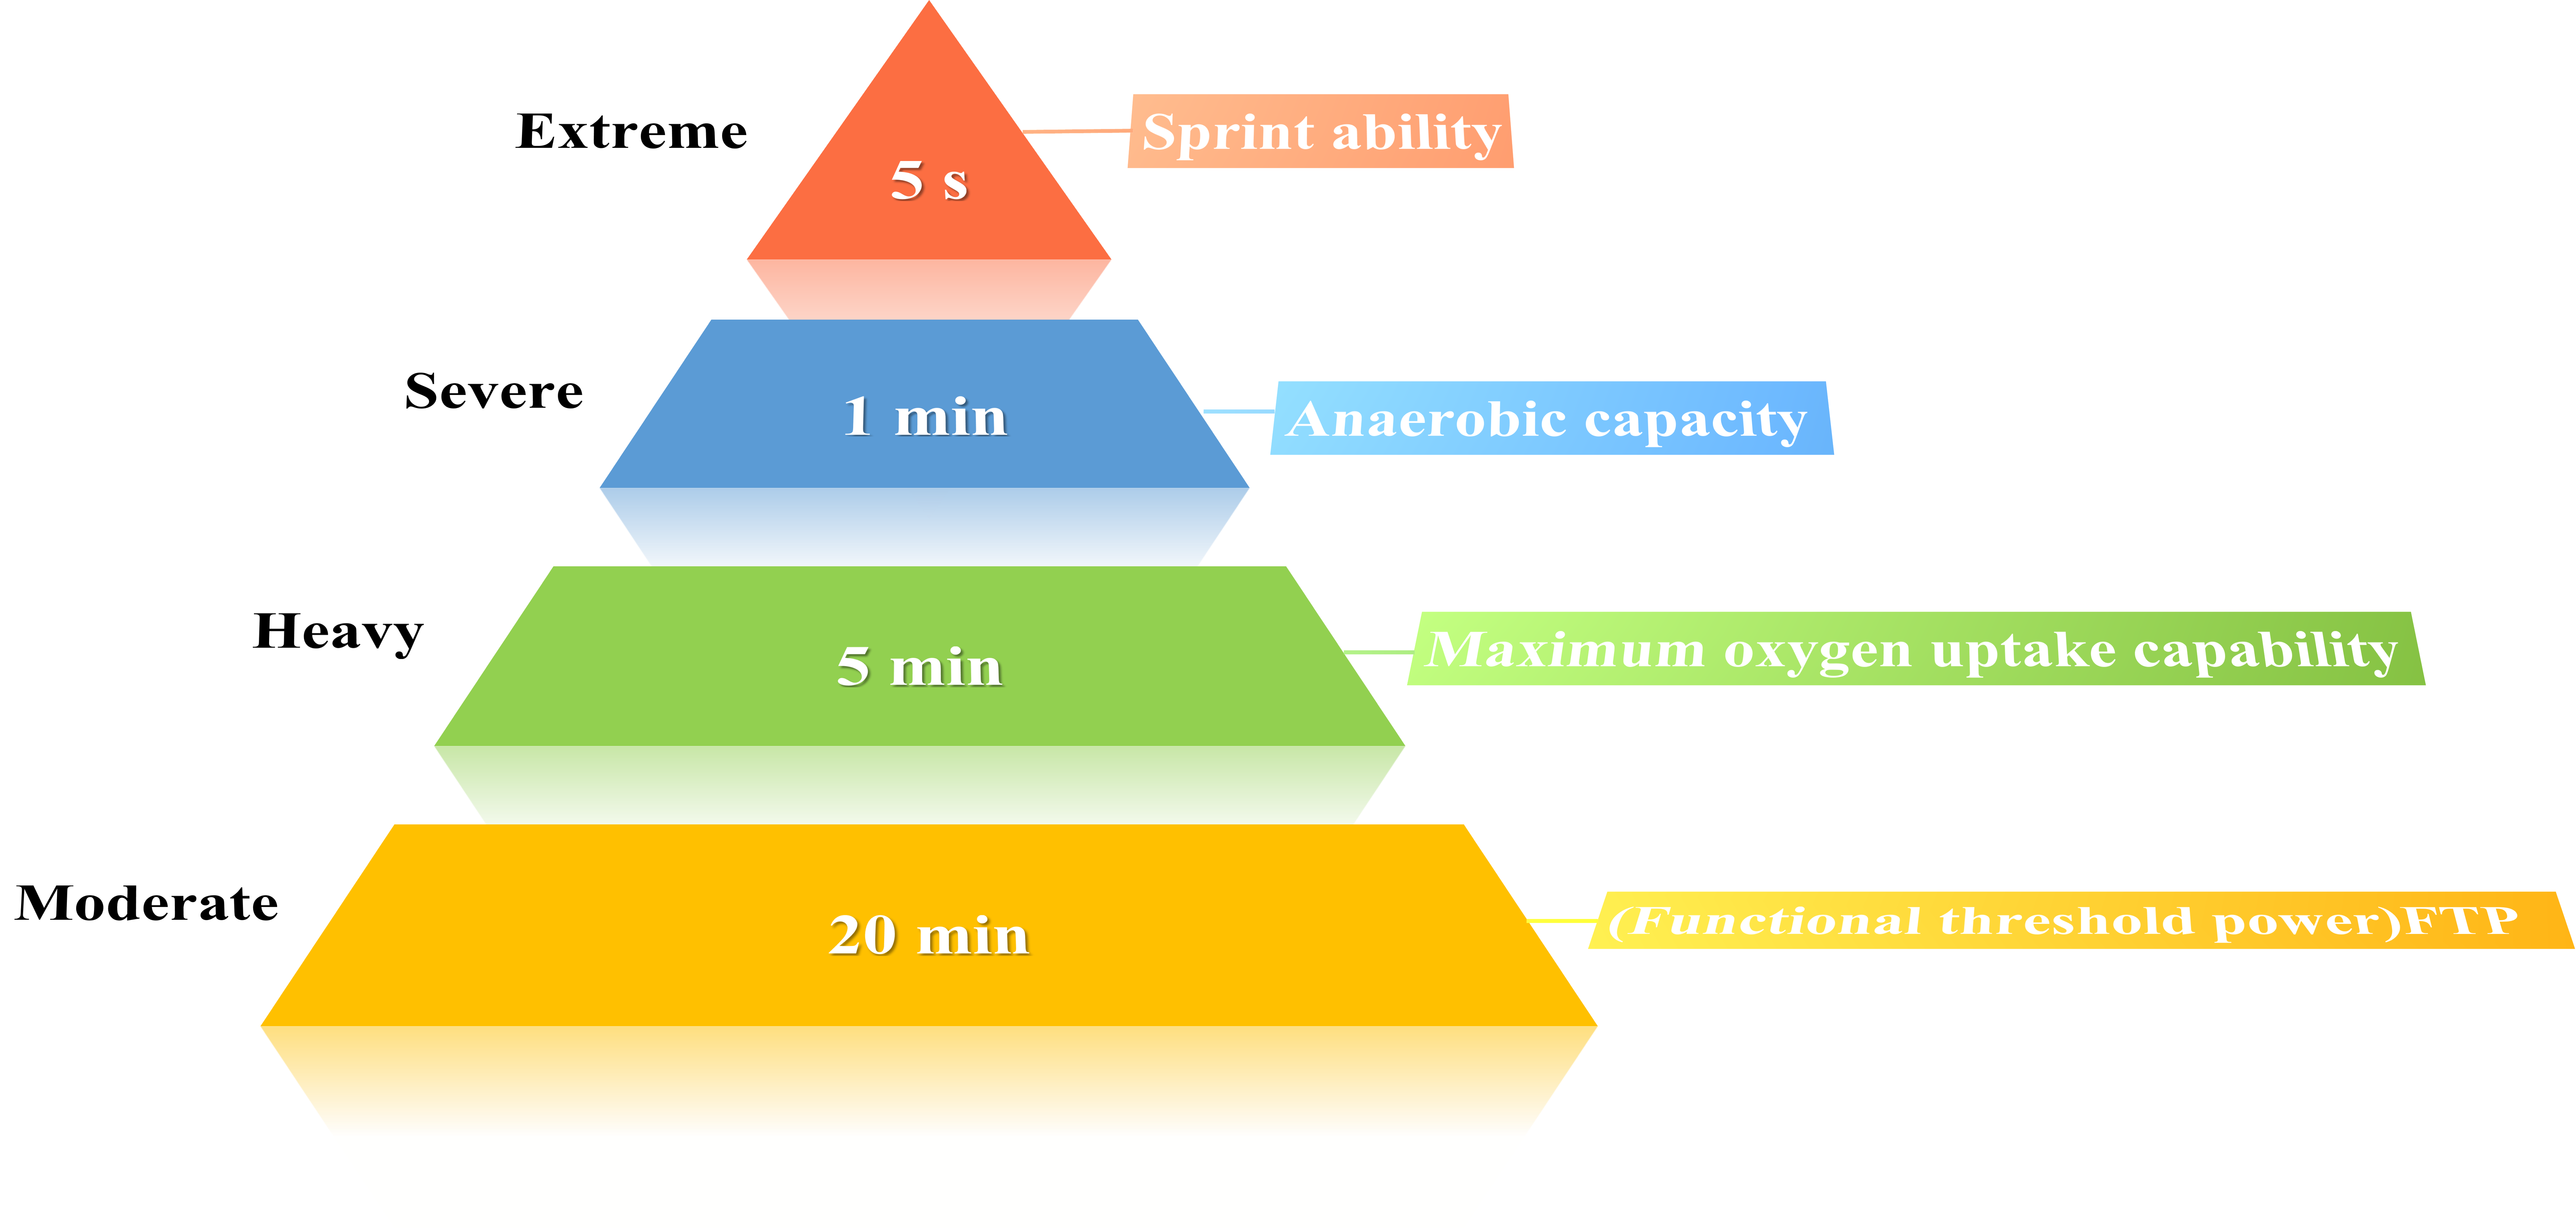
\includegraphics[width=0.9\linewidth]{image/pyramid}
\label{pyramid}
\end{wrapfigure}
	\par In this section, we establish the model of power curve, and consider people of different genders and types. 
	\par We first use the power profile chart to assess the ability of two types of rider briefly, which contains ability assessment in {\bf four domains}: {\bf extreme} intensity, {\bf severe} intensity, {\bf heavy} and {\bf moderate}, represented by {\bf 5s, 1 minute, 5 minutes and 20 minutes maximum power output} separately, as is shown on the left. Also, we plot the power curve of different athletes, showing the functional relationship  between maximal time and power output per weight. 
\subsection{Model Establishment}
In a gesture to have a general idea about the distribution of cycling levels, we turn to standard power profile and use the average cycling pace to plot the power curve. The dataset includes the riders' maximum power output during a certain period of time, ranging from novice to world-class, both men and women. Also, the power profile chart gives out the standard of different types, ensuring us to analyze the ability of riders in all domains of various types.
\par In the process of establishment, we discover that the profile of people of different levels, genders and rider types can vary greatly, that is to say, people of higher level have a better performance in all domains and sprinters do better in extreme intensity domain than time trialist and perform worse in other domains than TT.
\begin{figure}[h]
	\centering
	\begin{minipage}[t]{0.45\textwidth}
		\centering
		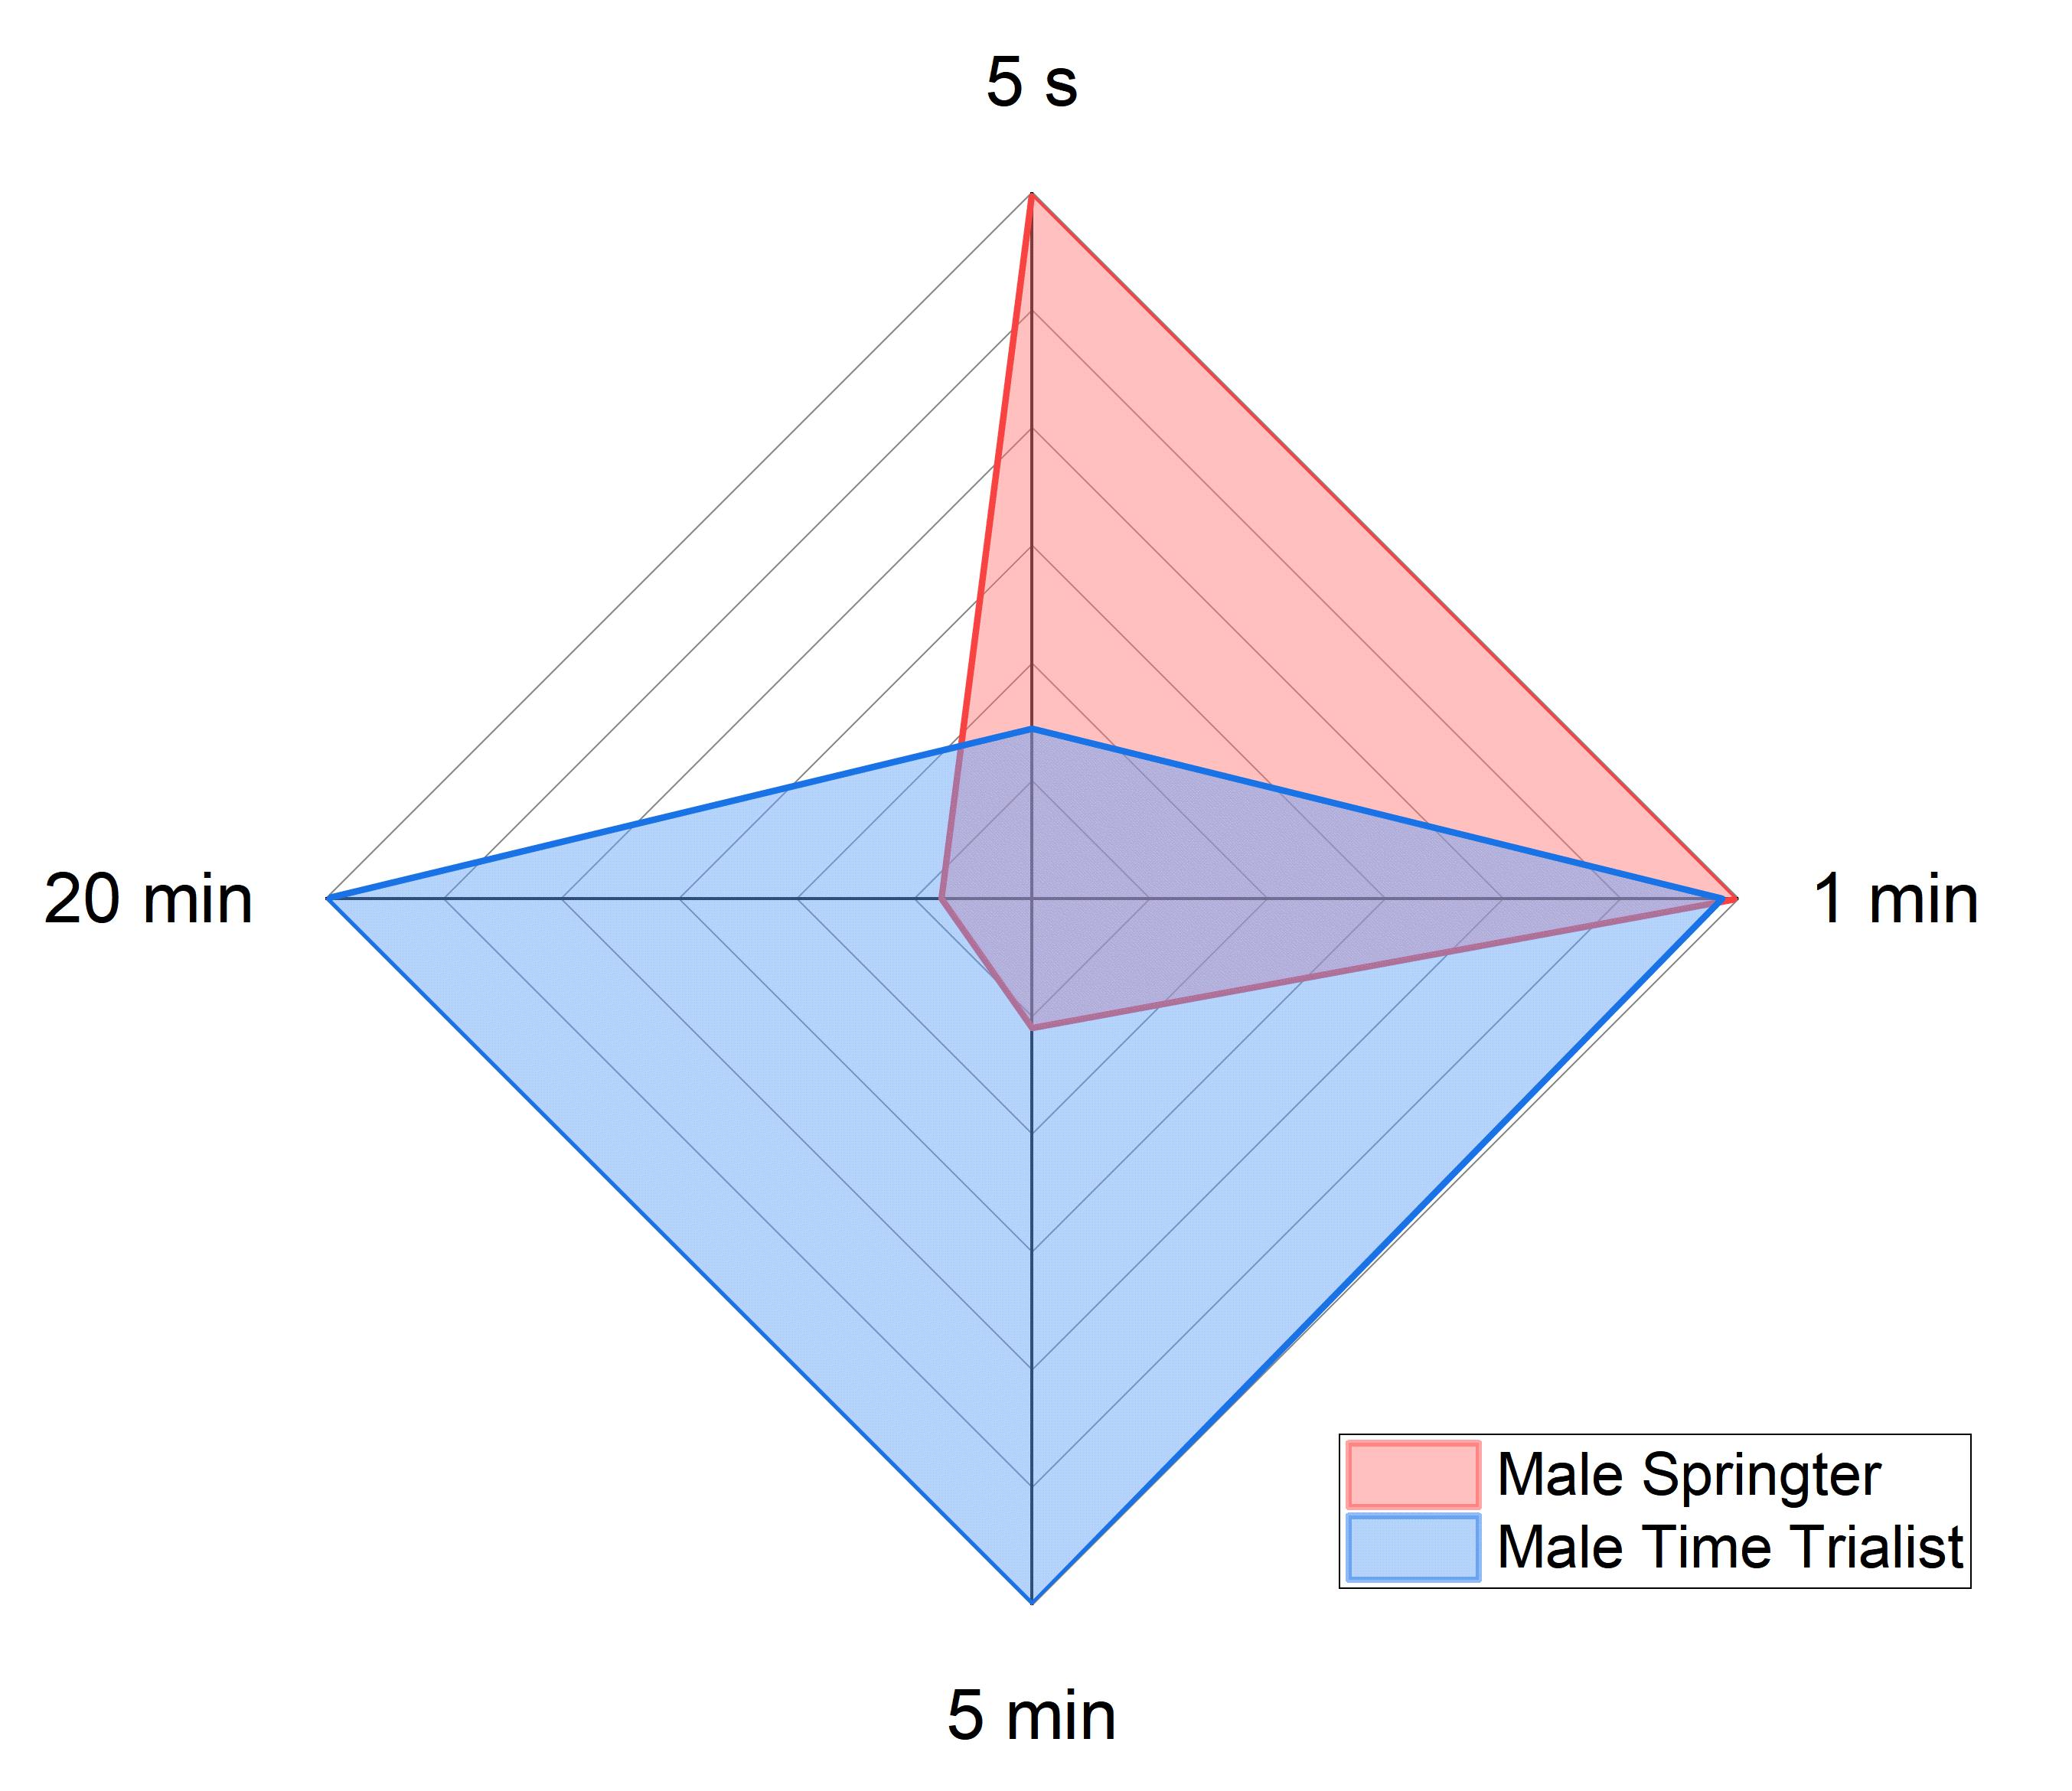
\includegraphics[width=0.7\linewidth]{image/radar/radar2}
		\caption{Radar map of male riders}
		\label{radar1}
	\end{minipage}
	\begin{minipage}[t]{0.45\textwidth}
		\centering
		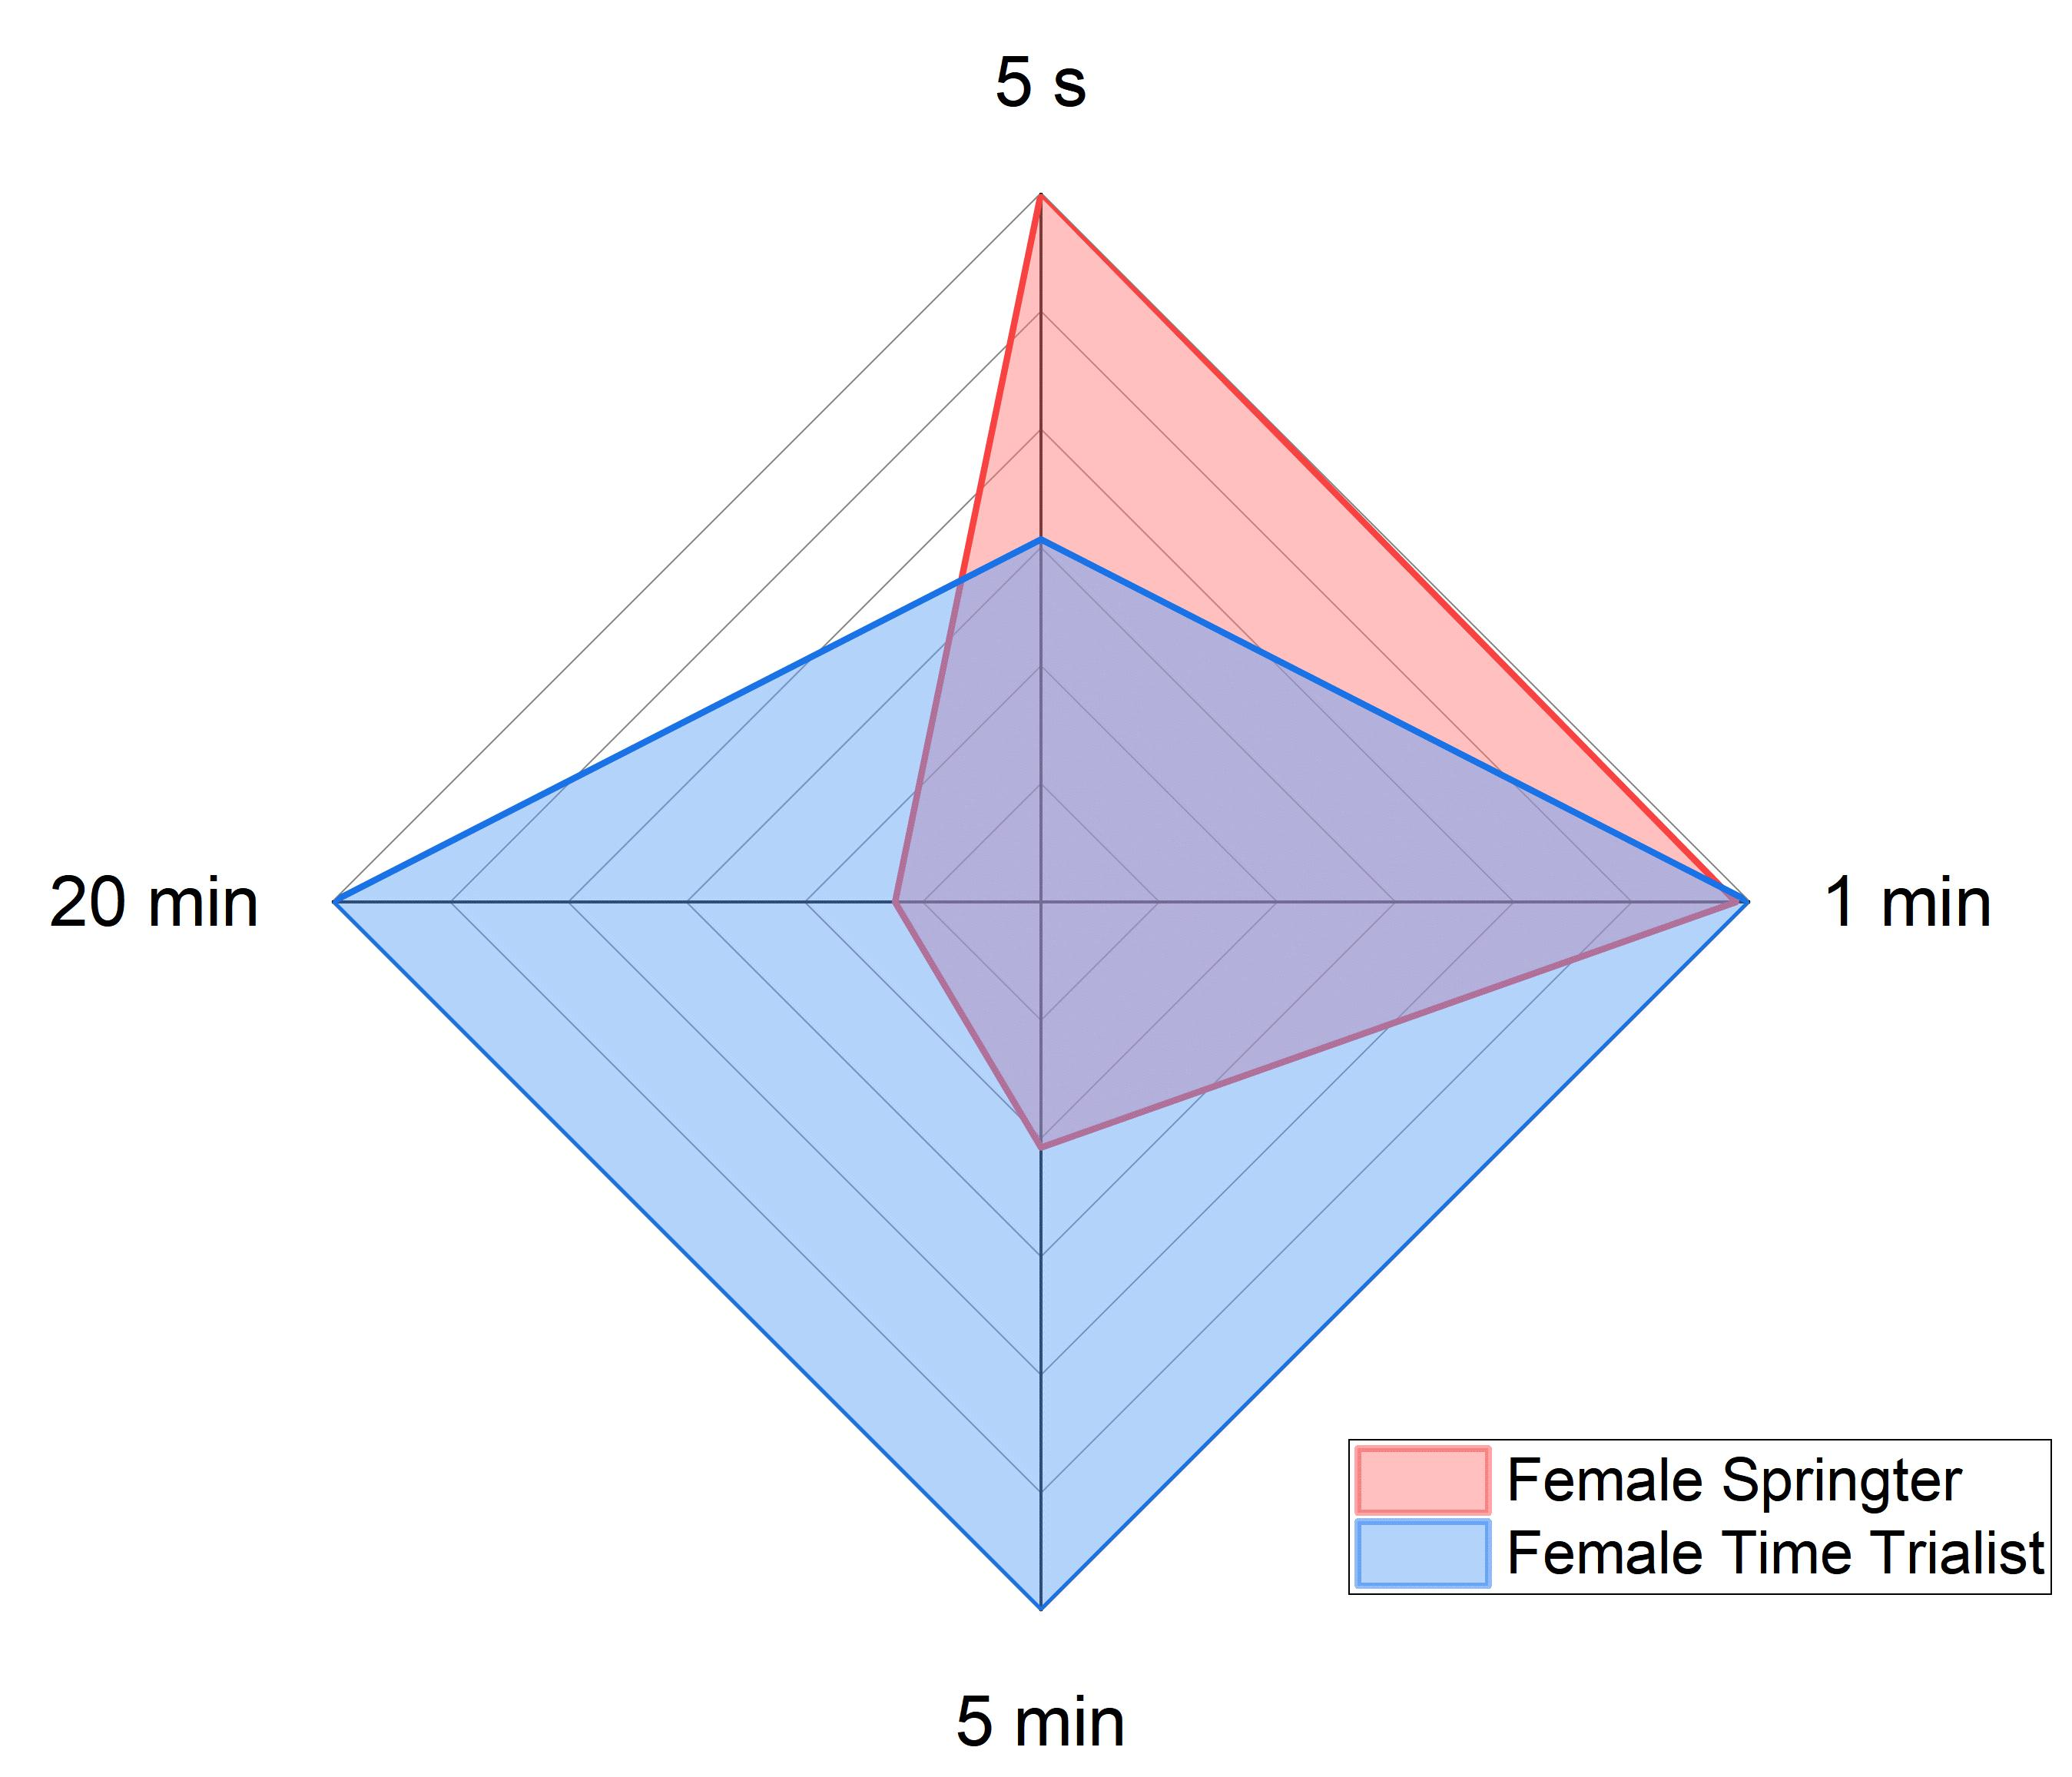
\includegraphics[width=0.7\linewidth]{image/radar/radar1}
		\caption{Radar map of female riders}
		\label{radar2}
	\end{minipage}
\end{figure}
\par As is shown in picture [\ref{radar1}][\ref{radar2}], sprinters  of both genders perform best in extreme intensity domain, while the two types of riders perform equally well in severe intensity domain. However, time trialists do much better in heavy and moderate domain.
\par With data from profile charts, we can sketch out the profile curve of different types of riders of different genders[\ref{sketch1}][\ref{sketch2}], and show their ability in four domains.
% TODO: \usepackage{graphicx} required
\begin{figure}[h]
	\centering
	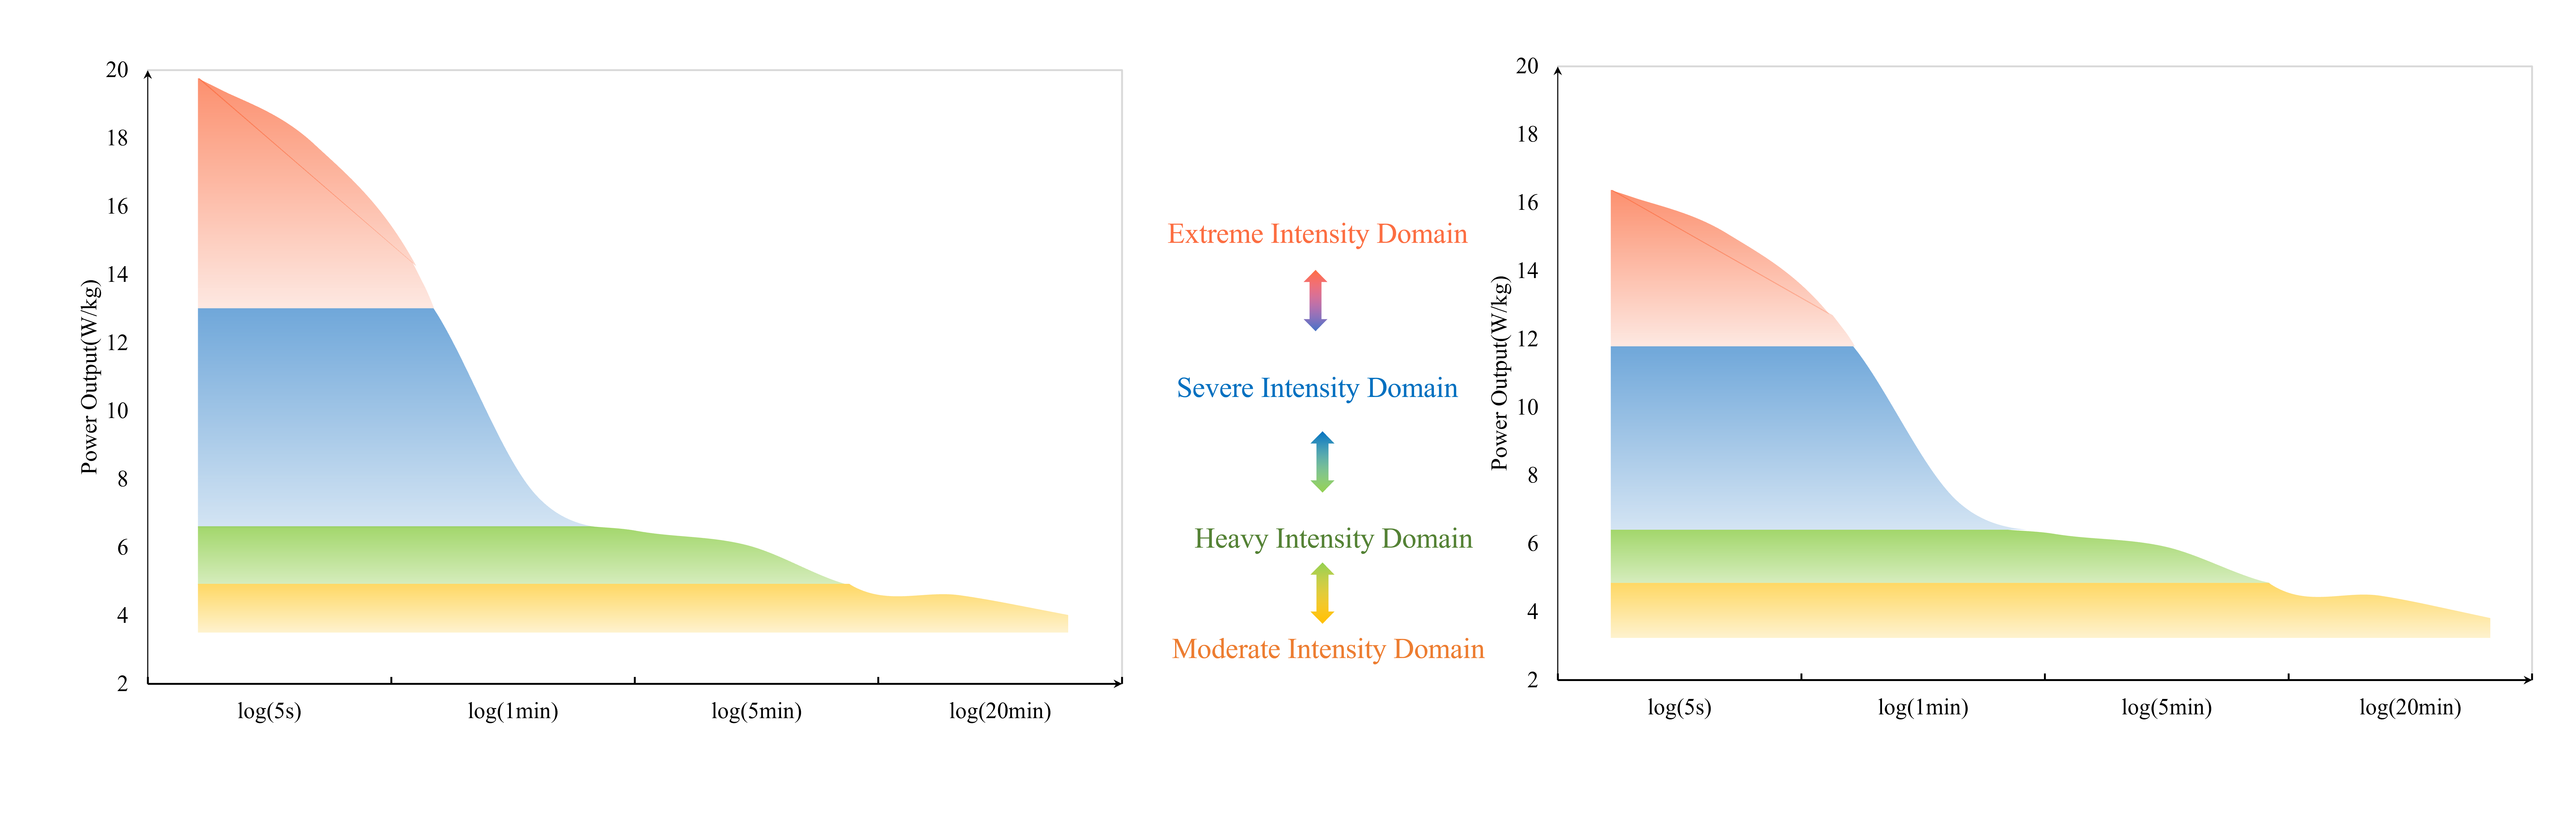
\includegraphics[width=1.0\linewidth]{image/sprinter}
	\caption{Sketch of power curve of male and female sprinters}
	\label{sketch1}
\end{figure}
% TODO: \usepackage{graphicx} required
\begin{figure}[h]
	\centering
	\includegraphics[width=1.0\linewidth]{"image/time trival"}
	\caption{Sketch of power curve of male and female time trialists}
	\label{sketch2}
\end{figure}

\par In order to reflect the distinction, we use the function to depict the relationship between power output per weight and time one man can maintain at that level:  
\begin{equation}
	\label{func}
	P=f(t)=at^b+c (b<0)
\end{equation}
The unknown parameters a and b represent different rider types and c represents different levels. For example, the function of sprinters have larger parameter of a and those who of world class have bigger c. In this sense, we name a and b as type parameter and c as level parameter.
\par In the next part, we will determine the value of parameters for functions of different rider types and genders to see whether the parameters will show how riders perform in different domains.

\subsection{Solution of Model}
With the help of power profile chart, we can easily obtain the ability level of an amateur, whose level is above-average. Then we use MATLAB to fit functions. 
\par As mentioned before, we use Eq (\ref{func}) to describe the relationship between power output per weight and the duration one cyclist can maintain at that level. Using data from power profile chart, we determine the value of three equations: style parameters a and b and level parameter c, as is shown in table [\ref{para:abc}].


\begin{table}[htbp]
	\setlength{\belowcaptionskip}{0.2cm}
	%\renewcommand\arraystretch{1.3}
	\setlength\tabcolsep{13pt}%调列距
	\centering
	\caption{Parameter estimation results}
	\begin{tabular}{cccc}
		\toprule[2pt]
		& {\bf a}     & {\bf b}     & {\bf c} \\
		\midrule
		Male's time trialist & 23.31 & -0.89 & 3.42 \\
		Male's sprinter & 36.62 & -0.98 & 1.56 \\
		Female's time trialist & 21.57 & -0.73 & 2.26 \\
		Female's sprinter & 26.82 & -0.74 & 0.27 \\
		\bottomrule[2pt]
	\end{tabular}%
	\label{para:abc}%
\end{table}%
%\par We use MATLAB to perform fitting to obtain four Power-Time-Energy equations.
\par With help of the results, we can easily obtain power curves of different athletes with putting parameters into Eq (\ref{func}).

\subsection{Analysis of Results}
As stated before, parameter a and b represent the style of an athlete and c reflects his level. As we can see from table [\ref{para:abc}], for men and women of the same style, parameter c of men is larger than that of women, which shows that the average physical strength of men is higher than that of women. With respect to different rider types, it's obvious that ability in extreme intensity domain of sprinters is larger than that of trialists, which means that sprinter's extreme exercise ability exceeds that of trialists.
Then we consider the goodness of fit in table [\ref{tab:sse}]:
\begin{table}[h]
%	\renewcommand\arraystretch{1.3}
	\setlength{\belowcaptionskip}{0.2cm}
	\setlength\tabcolsep{16pt}%调列距
	\centering
	\caption{Parameter estimation error}
\begin{tabular}{cccc}
\toprule[2pt]
& {\bf Sum of Squares Error(SSE) }  & {\bf Adjusted }$\bm{R^2}$ & {\bf RMSE} \\
\midrule
	MTT   & 0.3001  & 0.9879  & 0.5478  \\
	MSP   & 0.7471  & 0.9870  & 0.8644  \\
	FTT   & 0.2712  & 0.9881  & 0.5208  \\
	FSP   & 0.5641  & 0.9840  & 0.7511  \\
		\bottomrule[2pt]
\end{tabular}%

	\label{tab:sse}%
\end{table}%
\par Table above shows the partial result of variance analysis where values of adjusted $R^2$ are all above 0.98 and SSE values are nearly zero, indicating an excellent fitting effect in our model for 4 riders.
\section{Solution of the Second Problem}
\subsection{Model Establishment}
\par According to our assumptions, the cyclist's entire race is described as several segments of uniform motion: $\{(P_i,T_i)\},i=1,2,\cdots,N$, controlled by Power-Time-Energy Equation (PTE Equation):
\begin{equation}\label{PTE}
	\sum_{i=1}^N P_iT_i=\int_{\sigma }^{}E(s)ds 
\end{equation}
where $P_i$ denotes the average power per kilogram of the $i^{th}$ period, $T_i$ denotes the interval length of the $i^{th}$ time period, $E(s)$ denotes the energy consumed per kilogram per kilometer at the position of s, $\sigma$ represents the track curve.
\par Due to the limitations of the overall force of the athlete, $P_i$ needs to be subject to some constraints, which we describe as follows:
\begin{equation}\label{cons1}
\frac{1}{10} f^{-1}(P_i)\leq T_i \leq f^{-1}(P_i)
	\end{equation}
\begin{equation}\label{cons2}
	\begin{split}
		P_i > FTP \Leftrightarrow \left\{
	\begin{array}{rcl}
		P_{i-1}\leq FTP\\
		\quad \\
		T_{i} \leq \frac{W_i}{P_i-FTP}\\
		\quad\\
		W_i=\frac{C\ln T_{i-1}}{P_{i-1}+D}
	\end{array} \right.
\end{split}
\end{equation}
where $f$ is the power curve fitted from power profile, and it is a strictly monotonically decreasing function where $f^{-1}(P_i)$ denotes the maximum length of time a cyclist can maintain $P_i$-power.
\begin{wrapfigure}{l}{7cm} % 靠文字内容的左侧
	\includegraphics[width=0.6\linewidth]{image/w}
	\label{pyramid}
\end{wrapfigure}
\par Constraint (\ref{cons1}) points out that the length of each time period shall not be too small or too large, and the maximum is limited by the power curve. Constraint (\ref{cons2}) is the mechanism of recovery, which indicates that only if a cyclist stays below the FTP power for some time and restores the extra energy $W_i$ can he rides at a power above FTP in the next time period.

\par It must be pointed out that $E(s)$ may be affected by many factors, such as weather and road condition. We conclude the following mathematical model:

\begin{equation}
	\label{E}
	E(s) = \overline{E}(1-k_1v^2\cos\theta(s))(1+k_2\sin\phi(s))
\end{equation}
where $\overline{E}$ denotes the the energy consumed per kilometer under the windless condition of flat ground, $v$ is the speed of wind, $\theta(s)$ denotes the angle between the rider's direction and the wind at position of s, and $\phi(s)$ is the slope gradient, $k_1$ and $k_2$ are constants.

\par Eq (\ref{PTE}) together with Constraint (\ref{cons1})( \ref{cons2}) makes up the model which describes the competition process.

\par When having both rider information (Power Profile \& Power Curve) and track information (each $E(s)$), it is possible to construct Optimizer to produce the best strategy for a rider. We assume that a cyclist's entire race schedule is divided into three parts: the FTP stage ($P_1,T_1$), the recovery stage ($P_2,T_2$), and the sprint stage ($P_3,T_3$), with power equal to, less than, and greater than FTP.
\par The objective function of optimization is $T_1+T_2+T_3$. Eq (\ref{PTE}) and Constraint (\ref{cons1}) (\ref{cons2}) make up the constraints. The model of Optimizer is described as follows:

\begin{equation}
	\min T_1+T_2+T_3 \quad\quad \rm{s.t.}
	\label{min}
\end{equation}

\begin{equation}\label{cons3}
\begin{split}
		\left\{
		\begin{aligned}
		%	\begin{array}{rcl}
				&\sum_{i=1}^{3}P_iT_i= \int_{\sigma }^{}E(s)ds \\
				\quad \\
			&\frac{1}{10} f^{-1}(P_i)\leq T_i \leq f^{-1}(P_i)\\
				\quad\\
				&P_1=FTP,P_2<FTP,P_3>FTP\\
				\quad \\
				&T_3 \le ({\frac{\ln T_2}{p_2+D}+C})/{(P_3-FTP)}\\
				\end{aligned}
		%	\end{array} 
	\right.
\end{split}
\end{equation}
\par By consulting the literature and parameter estimation, we determined that $C=700,D=0.33,\overline{E}=0.44$.
\par To solve the optimization problem, we use the fmincon function in MATLAB, which aims to find the minimum of a constrained nonlinear multivariate function. This function include four methods: interior-point, sqp, active-set, trust-region-reflective.

\subsection{Application of Model}

\par To apply the model to real-world competitions, we construct two world-class virtual time trialists: MTT (Male Time Trialist) and FTT (Female Time Trialist), together with their power profiles. Then we use the model to simulate the process of their participation in real-world competitions. After finding the best tactic through numerical optimization, their results will be compared with real-world competitors.

\par Power profiles of MTT and FTT are listed as table [\ref{tab:pp}]:
% Table generated by Excel2LaTeX from sheet 'timetrialist'
% Table generated by Excel2LaTeX from sheet 'timetrialist'
\begin{table}[htbp]
	%	\renewcommand\arraystretch{1.3}
	\setlength{\belowcaptionskip}{0.2cm}
	%\setlength\tabcolsep{16pt}%调列距
	\centering
	\caption{ Power Profiles of MTT and FTT}
	\begin{tabular}{c|cccc|cccc}
		\toprule[2pt]
		& \multicolumn{4}{c|}{MTT}      & \multicolumn{4}{c}{FTT} \\
		\midrule
		maximum duration & 5 s   & 1 min & 5 min & FT    & 5 s   & 1 min & 5 min & FT \\
		power output(W/kg) & 19.69 & 10.01 & 6.98  & 6.40  & 17.48 & 9.29  & 6.33  & 5.61 \\
		\bottomrule[2pt]
	\end{tabular}%
	\label{tab:pp}%
\end{table}%

\subsubsection{2021 Olympic Time Trial course in Tokyo}
% TODO: \usepackage{graphicx} required
\begin{figure}[h]
	\centering
	\includegraphics[width=0.8\linewidth]{"image/东京+uci/东京 女 time trial circuit"}
	\caption{Topographic profile of 2021 Olympic Time Trial course in Tokyo}
	\label{trackt}
\end{figure}
\paragraph{} Tracks of 2021 Olympic Time Trial in Tokyo are both around Mount Fuji, and both courses have a lot of elevation fluctuations. The women will complete one full lap for a total of 22.1 kilometers with a total elevation gain of 423 meters[\ref{trackt}], and the men cover a distance of 44.2 kilometers, which is two laps around the women's track.

\par We use the power profile of MTT and FTT, and we apply our model to this course. As the terrain of the course is very undulating, it's hard to ignore the effects of altitude changes on athletes, so we take it into account. With the help of our model, we get the minimum time to cover the distance for to virtual athletes, shown in table [\ref{time}].
% Table generated by Excel2LaTeX from sheet 'Sheet2'
\begin{table}[htbp]
	%	\renewcommand\arraystretch{1.3}
	\setlength{\belowcaptionskip}{0.2cm}
	\setlength\tabcolsep{16pt}%调列距
	\centering
	\caption{ Minimum time to finish OITT}
	\begin{tabular}{ccccc}
		\toprule[2pt]
		&$ T_1$(min)    & $T_2$(min)    & $T_3$ (min)   & Total(min) \\
		\midrule
		MTT   & 28:41 & 21:15 & 7:16  & 57:12\\
		FTT   & 22:39 & 3:17  & 8:42  & 34:38\\
		\bottomrule[2pt]
	\end{tabular}%
	\label{time}%
\end{table}%
\par As is shown in table [\ref{time}], the virtual male rider exerts his strength at the level of FTP in the first 28:41(min), and recover for 21:16(min), controlling his average power output per kg at 6.40 W/kg. in the final sprint, he exerts all effort over the level of FTP, maintaining 7.16 power output per kg, and finally scores 57:12(min). The same goes for the analysis of women, whose power output per kg is FTP, 5.61 and 6.34 separately.
\par In order to verify the correctness of the model, we compare the score of  MTT with that of three riders who participated in 2021 Olympic Time Trial, and find that our MTT and FTT rider rank 7 and 23 separately. As our data simulates the level of world athletes, our optimization results are reliable.
% TODO: \usepackage{graphicx} required
\begin{figure}[h]
	\centering
	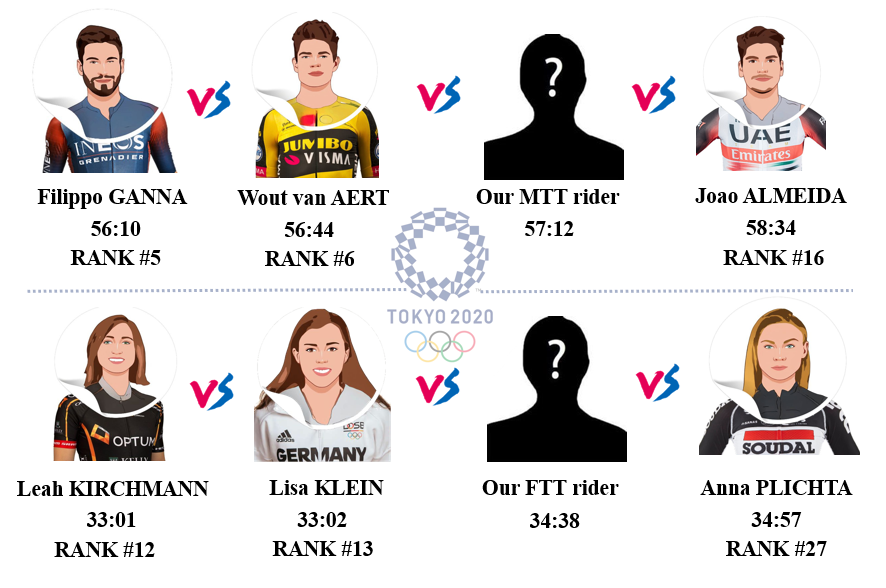
\includegraphics[width=0.8\linewidth]{image/tkyo}
	\caption{Our virtual riders and participants of 2021 Olympic Time Trial}
	\label{tkyo}
\end{figure}
 
\subsubsection{2021 UCI World Championship time trial course in Flanders}
\paragraph{} The start of 2021 UCI World Championship time trial is situated on the North Sea beach for both men and woman elite. The women will complete course for a total of 30.30 kilometers with a total elevation gain of 54 meters and men need to finish additional lap for 13 kilometers and elevation gain of 24 meters compared with women's. The whole course is relatively flat which belongs to Cat 4 comparing with Hors Catégorie. Therefore, the energy consumption per kilometer is considered the same under the windless condition on flat ground, which means $E(s)$ always equals $\overline{E}$.
\par By applying our model, we obtain the minimum time to finish race for virtual athletes, shown in table [\ref{time2}].
\begin{table}[h]
	%	\renewcommand\arraystretch{1.3}
	\setlength{\belowcaptionskip}{0.2cm}
	\setlength\tabcolsep{16pt}%调列距
	\centering
	\caption{ Minimum time to finish UCI WCTT}
	\begin{tabular}{ccccc}
		\toprule[2pt]
		&$ T_1$(min)    & $T_2$(min)    & $T_3$ (min)   & Total(min) \\
		\midrule
		MTT   & 27:23 & 15:07 & 7:05  & 49:35 \\
		FTT   & 26:21 & 3:17  & 8:49  & 38:27 \\
		\bottomrule[2pt]
	\end{tabular}%
	\label{time2}%
\end{table}%

\par As is shown in table [\ref{time2}], our virtual male cyclist applies power at the level of FTP in the first 27:23(min), the recovers for 14:07(min)and finally makes all-out effort to the end. His total result is 48:36(min). Results of female cyclist can be interpreted similarly.
\begin{figure}[h]
	\centering
	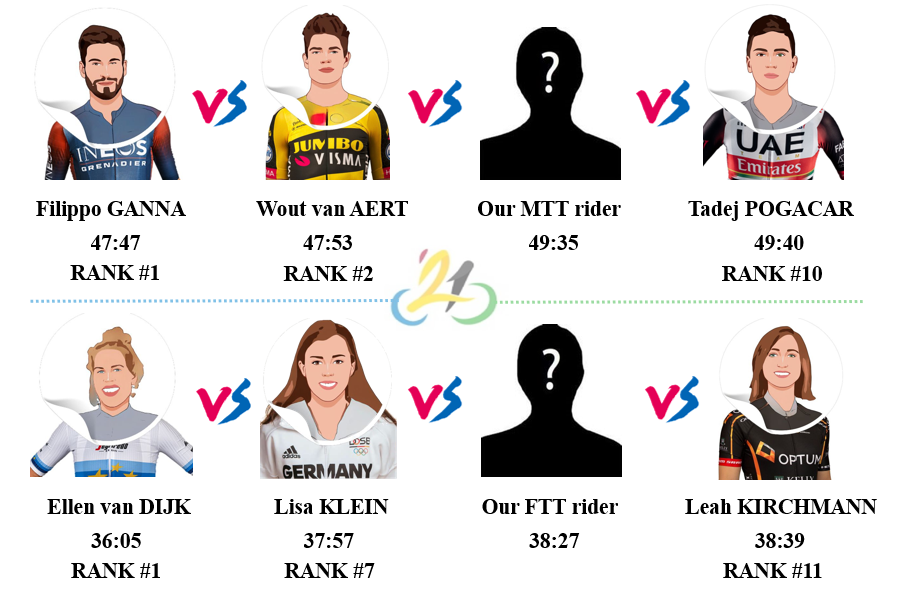
\includegraphics[width=0.9\linewidth]{image/rider1}
	\caption{Our virtual riders and participants of 2021 UCI World Championship time trial}
	\label{rider1}
\end{figure}
\par In order to verify the rationality and reliability of our model, we compare the score with ITT racers in 2021 UCI World Championship time trial as the graph presented [\ref{rider1}]---our MTT and FTT rider rank 5 and 10 respectivly.
% TODO: \usepackage{graphicx} required


\subsubsection{Self-designed course}

\paragraph{} By researching and sifting through a large number of cycling routes, we optimize one route which satisfies almost every requirements\footnote{https://www.strava.com/activities/1178477346/overview}. This course [\ref{route}] is located in Berkeley, USA, passing through Greezly Peak and Berkeley Hills and finanlly ending up back at Berkeley. Riders will complete this course with many sharp curves and nontrivial road grades for a total of 28.26 kilometers with a total elevation gain of 564 meters.
% TODO: \usepackage{graphicx} required
\begin{figure}[h]
	\centering
	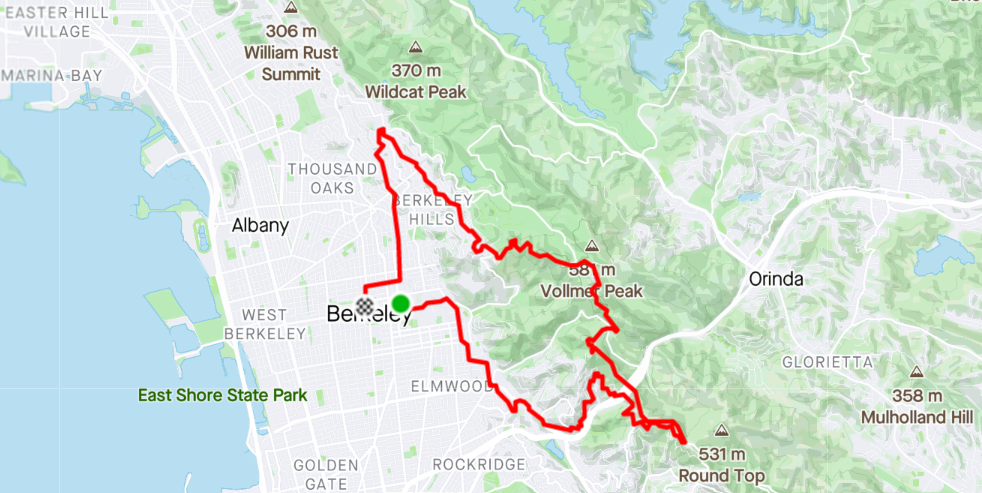
\includegraphics[width=1\linewidth]{image/route}
	\caption{Self-designed route}
	\label{route}
\end{figure}

\par From the circuit profile, after setting off, riders will head on a continuous uphill reaching 4.5 per cent gradient on average[\ref{self1}]. Then, the rolling roads include other climbs which are gentler than the previous course. After reaching the peak, riders will face downhill of almost 10 kilometers along the twists and turns to the finish.
% TODO: \usepackage{graphicx} required
\begin{figure}[h]
	\centering
	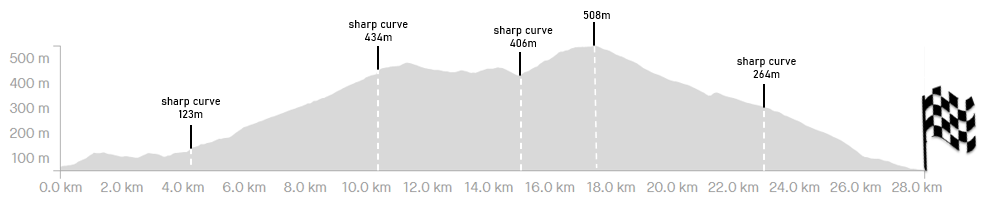
\includegraphics[width=0.9\linewidth]{image/self1}
	\caption{Topographic profile of self-designed course}
	\label{self1}
\end{figure}
\par By applying our model into our self-designed route, the optimal ride planning can be derived [\ref{time3}]. 
\begin{table}[h]
	%	\renewcommand\arraystretch{1.3}
	\setlength{\belowcaptionskip}{0.2cm}
	\setlength\tabcolsep{16pt}%调列距
	\centering
	\caption{ Minimum time to finish self-designed course}
	\begin{tabular}{ccccc}
		\toprule[2pt]
		&$ T_1$(min)    & $T_2$(min)    & $T_3$ (min)   & Total(min) \\
		\midrule
    MTT   & 28:51 & 5:37  & 7:14  & 41:42 \\
FTT   & 32:55 & 5:41  & 8:49  & 47:25 \\
\bottomrule[2pt]
\end{tabular}%
\label{time3}%
\end{table}%
\par Also, an amateur completed the track and uploaded his ride stats on the website. We compare the simulated data to his ride data [\ref{rider3}], and find that the rider lags behind our MTT and FTT riders. It's easy to explain: our riders are world-class athletes, while the strava user is an  amateur. As a result, our model can be correctly applied and proved again. 
% TODO: \usepackage{graphicx} required
\begin{figure}[h]
	\centering
	
\includegraphics[width=0.7\linewidth]{image/rider3}
	\caption{Our virtual riders and participants of self-designed time trial}
	\label{rider3}
\end{figure}

\section{Sensitivity Analysis of Weather Conditions}
\subsection{Impact of Wind Direction}

\par In order to characterize the effect of wind direction on the model, we will establish and prove {\bf Wind Direction Theorem}, which indicates that under certain conditions, the wind direction has no effect on the closed circular bicycle track. 

\par Eliminating the effect of slope, $E_j$ can be described as follows according to Eq (\ref{E}):

\begin{equation}
	E(s) = \overline{E}(1-k_1v^2\cos\theta(s))
\end{equation}
\begin{flushleft}
\par where $v$ is wind speed, a constant according to our assumption.
\end{flushleft}
% TODO: \usepackage{graphicx} required

\begin{wrapfigure}{l}{9cm} 
	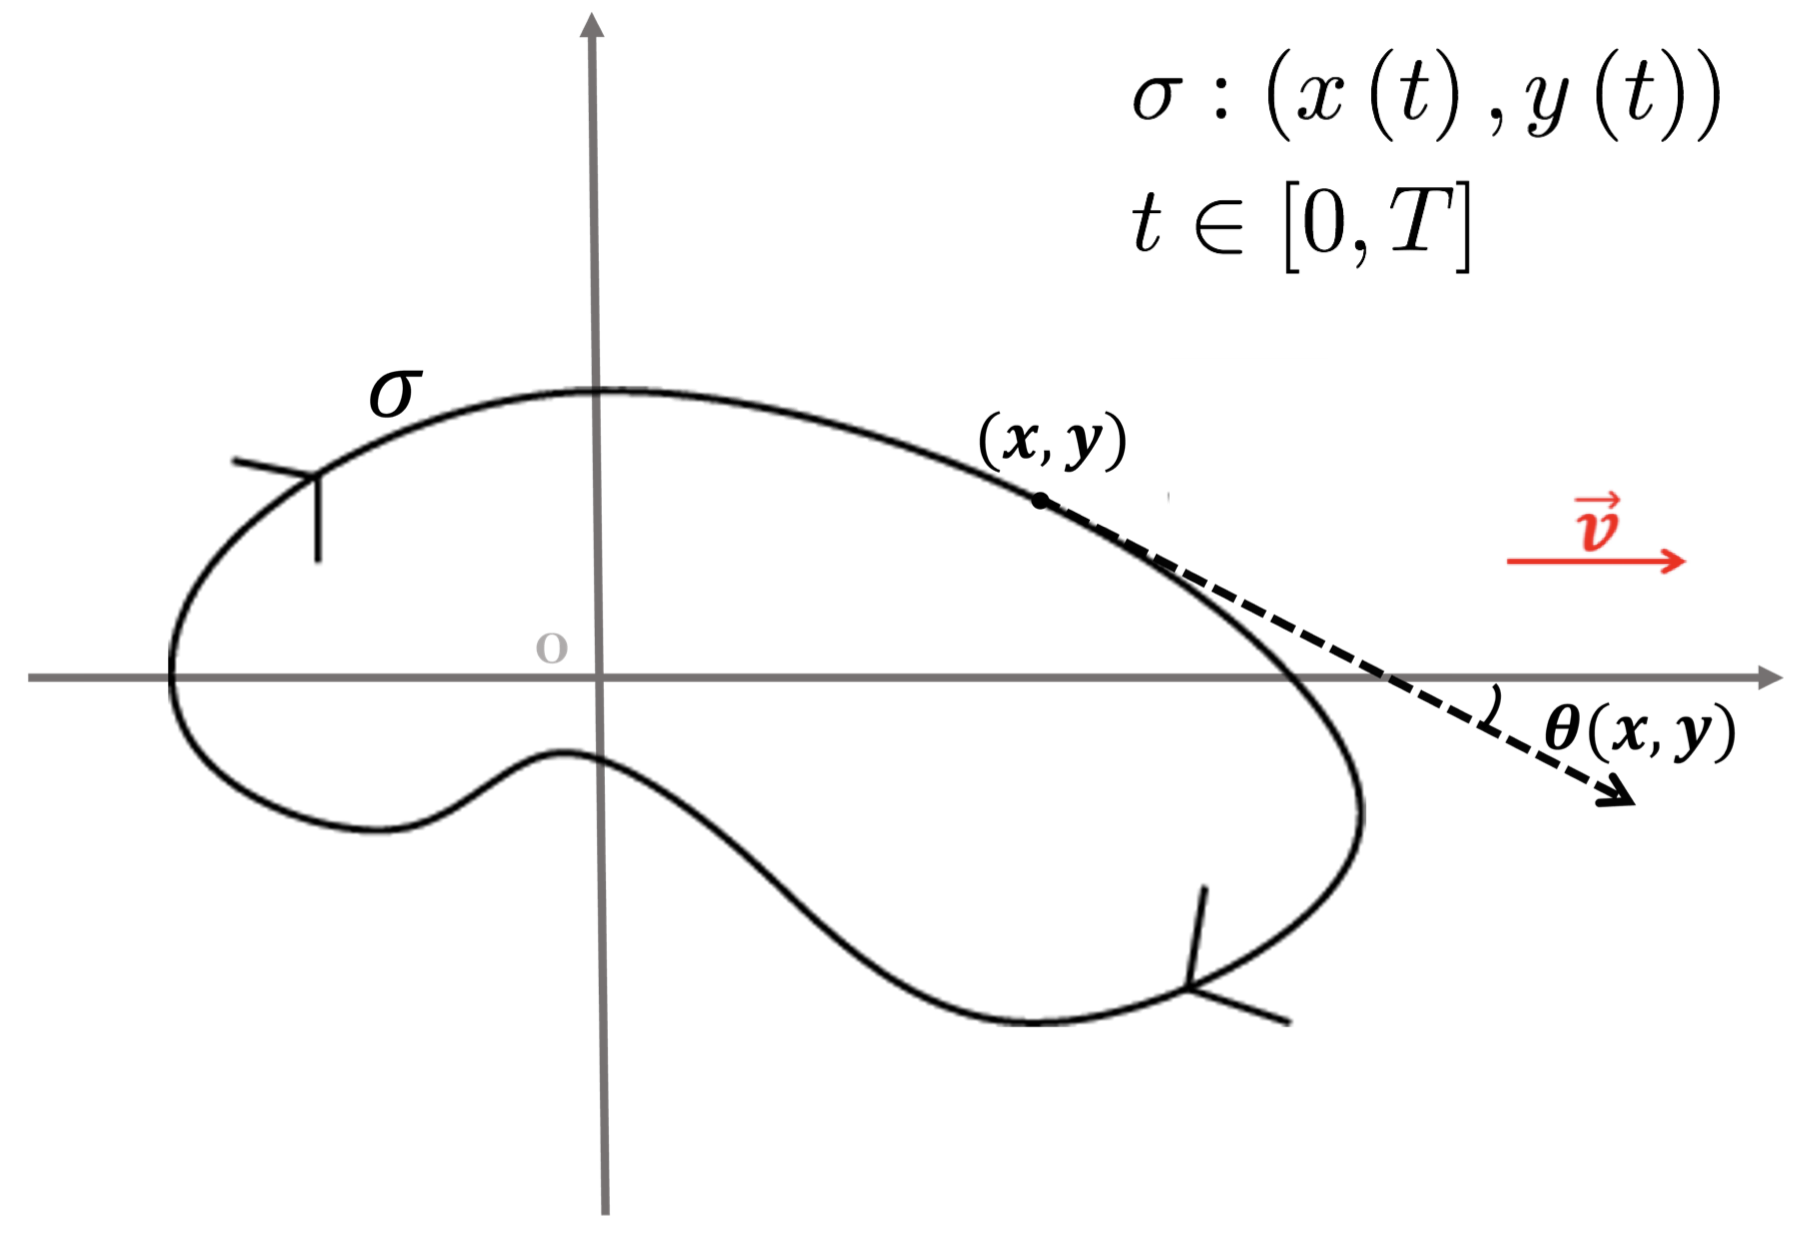
\includegraphics[width=0.7\linewidth]{image/fig3}
	\label{fig3}
\end{wrapfigure}

 \par A plane rectangular coordinate system is established with the wind direction as positive direction of the x-axis. Note that the circular track $\sigma$ is a $C^1$ (first-order continuously differentiable) closed curve in the plane with parametric equation as left.

{\bf Theorem 1 (Wind Direction Theorem) :} If $\sigma$ is a $C^1$ closed curve, then
\begin{equation}\label{WDT}
	\int_{\sigma} \overline{E}(1-k_1v^2\cos\theta)ds = \int_{\sigma} \overline{E} ds
\end{equation}
 where $\theta=\theta(x,y)=y'(t)/x'(t)$ denotes the angle between the tangent at $(x,y)$ and the x-axis. 
\begin{proof}[Proof:]

\begin{equation}
	\begin{aligned}
	\int_{\sigma} \overline{E}(1-k_1v^2\cos\theta)ds - \int_{\sigma} \overline{E} ds
	&= -\overline{E}k_1v^2 \int_{\sigma} \cos\theta(x,y) ds\\
	&= -\overline{E}k_1v^2 \int_0^T \frac{\sqrt{x'(t)^2+y'(t)^2}}{\sqrt{1+(\frac{y'(t)}{x'(t)})^2}} dt\\
	&= -\overline{E}k_1v^2 \int_0^T x'(t) dt\\
	&= -\overline{E}k_1v^2 (x(T)-x(0))\\
	&= 0
\end{aligned}
\end{equation}
\par For $\sigma$ is a closed curve, $x(T)=x(0)$. The variable substitution formula of the first type curve integral is used at the second equal sign.
\end{proof}
\begin{flushleft}
	\qquad Wind Direction Theorem implies that the effect of wind direction on the total energy (per kilometer) required to complete the race is only relevant to the start and finish, instead of the condition of each track. The mathematical explanation is presented below:
\end{flushleft}
\begin{wrapfigure}{l}{5cm} % 靠文字内容的左侧
	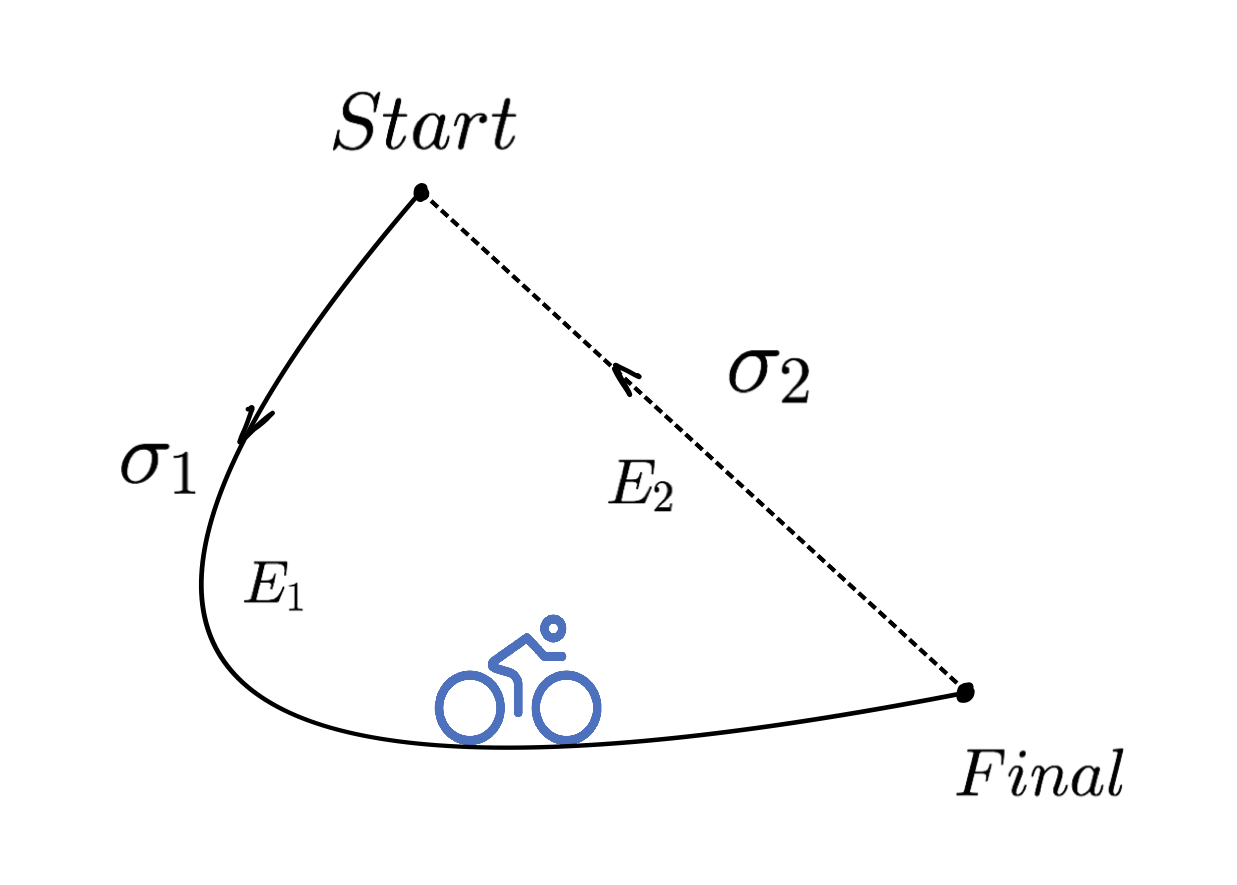
\includegraphics[width=0.8\linewidth]{image/fig1}
	\label{fig1}
\end{wrapfigure}
  \par The track is represented by $\sigma_1$, and $\sigma_2$ denotes the line connecting start and final. Let $E_i(s)$ become the energy cost per kilometer at position $s$ on $\sigma_i$ while there exists wind, and $\Delta E_i=\int_{\sigma_i}(E_i(s)-\overline{E})ds$. 
\par According to Wind Direction Theorem, it is true that
\begin{equation}
	\int_{\sigma_1}E_1(s)ds + \int_{\sigma_2}E_2(s)ds = \overline{E} \int_{\sigma_1+\sigma_2}1ds.
\end{equation}
\par That is to say, $\Delta E_1 = -\Delta E_2$. And since $\sigma_2$ is a straight line, $\Delta E_2$ can be easily calculated by $-\overline{E}k_1v^2\cos\theta L_2$ ($L_2$ is the distance).
\par In conclusion, Wind Direction Theorem and its corollary indicate that wind direction and speed do not affect the total energy cost of a closed circular track. In non-closed cases, the change in total cost of energy can be calculated by start and end points, wind speed and direction.
\subsection{Impact of Wind Speed}
As discussed before, increase or decrease in total energy consumption due to wind is only related to wind speed, starting and end position. So in this part, we only talk about a non -closed route: UCI World Championship time trial course in Flanders.
\par Take UCI World Championship time trial course for men as an example, the straight line distance between start and end points can be calculated easily, which is important to the analysis of wind effect.
\par As discussed above, $E(s)$ can be described as follows according to Eq (\ref{E}):
\begin{equation}
	E(s) = \overline{E}(1-k_1v^2\cos\theta(s))
\end{equation}
where $v$ is a constant wind speed. 
\par Using our virtual rider MTT and FTT, we can simulate the model of this track at different wind speeds and solve out the optimal strategy. Then we can get results as table [\ref{wind}][\ref{wind2}].
% Table generated by Excel2LaTeX from sheet 'Male'
\begin{table}[h]
	%	\renewcommand\arraystretch{1.3}
	\setlength\tabcolsep{13pt}%调列距
	\setlength{\belowcaptionskip}{0.2cm}
	\centering
	\caption{Minimum time for men to finish UCI WCTT under weather condition}
	\begin{tabular}{c|ccccc}
		\toprule[2pt]
		& Wind Speed & $T_1$  & $T_2$  & $T_3$  & Total \\
		\midrule
		\multirow{2}[2]{*}{Downwind} & 15 mph    & 28:51 & 7:19  & 7:14  & 43:24 \\
		& 5 mph    & 28:51 & 9:56  & 7:14  & 46:01 \\
		\midrule
		No wind & 0     & 28:51 & 12:40 & 7:14  & 48:45 \\
		\midrule
		\multirow{2}[2]{*}{Upwind} & 5 mph     & 28:51 & 15:08 & 7:14  & 51:13 \\
		& 15 mph     & 28:51 & 17:44 & 7:14  & 53:49 \\
		\bottomrule[2pt]
	\end{tabular}%
	\label{wind}%
\end{table}%

% Table generated by Excel2LaTeX from sheet 'Female'
\begin{table}[h]
%	\renewcommand\arraystretch{1.3}
	\setlength\tabcolsep{13pt}%调列距
	\setlength{\belowcaptionskip}{0.2cm}
	\centering
	\caption{Minimum time for women to finish UCI WCTT under weather condition}
	\begin{tabular}{c|ccccc}
		\toprule[2pt]
		& Wind Speed & $T_1$  & $T_2$  & $T_3$  & Total \\
		\midrule
		\multirow{2}[2]{*}{Downwind} & 15 mph    & 19:25 & 3:17  & 8:49  & 31:31 \\
		& 5 mph    & 22:22 & 3:19  & 8:49  & 34:30 \\
		\midrule
		No wind & 0     & 26:20 & 3:18  & 8:49  & 38:27 \\
		\midrule
		\multirow{2}[2]{*}{Upwind} & 5 mph     & 28:19 & 3:18  & 8:49  & 40:26 \\
		& 15 mph     & 31:17 & 3:18  & 8:49  & 43:24 \\
		\bottomrule[2pt]
	\end{tabular}%
	\label{wind2}%
\end{table}%
\par We can conclude from the table that male riders will change the duration of recovery according to weather condition, while female riders will change FTP time($T_1$).
\par In all conditions, the virtual male rider exerts his strength at the level of FTP in the first period  $T_1$, and recover for 21:16(min), controlling his average power output per kg at 6.40 W/kg. In the final sprint, he exerts all effort over the level of FTP, maintaining 7.16 power output per kg, and finally scores 57:12(min). The same goes for the analysis of women, whose power output per kg is FTP, 5.61 and 6.34 separately.


\section{Sensitivity Analysis of Power Output}

Because in real life, it is difficult for athletes to precisely control the riding speed, let alone the output power. As a result, we need to consider the sensitivity of the model, especially the output power.
% Table generated by Excel2LaTeX from sheet 'Sheet1'
\begin{table}[h]
%		\renewcommand\arraystretch{0.9}
	\setlength\tabcolsep{13pt}%调列距
	\setlength{\belowcaptionskip}{0.2cm}
	\centering
	\caption{Strategies under different constraints for male}
	\begin{tabular}{ccc|cccc}
		\toprule[2pt]
		$P_1$    & $P_2$    & $P_3$    & $T_1$    & $T_2$    & $T_3$    & Total Time \\
		\midrule
		FTP   & 6.40  & 7.16  & 28:51 & 12:39 & 7:40  & 48:45 \\
		FTP   & \textbf{6.20 } & 6.76  & 28:51 & 6:58  & 13:14 & 49:04 \\
		FTP   & \textbf{6.00 } & 7.08  & 28:51 & 12:32 & 8:09  & 49:32 \\
		FTP   & 6.40  & \textbf{7.50 } & 28:51 & 15:04 & 4:51  & 48:46 \\
		FTP   & 6.40  & \textbf{8.00 } & 28:51 & 16:59 & 3:01  & 48:51 \\
		\bottomrule[2pt]
	\end{tabular}%
	\label{div}%
\end{table}%
\par In order to perform a sensitivity analysis, we change the parameter of power output for MTT, requiring the three stages of PO per kilogram to be constrained at a certain level. With new constraints, we get new results as table [\ref{div}].
% TODO: \usepackage{graphicx} required
\begin{figure}[h]
	\centering
	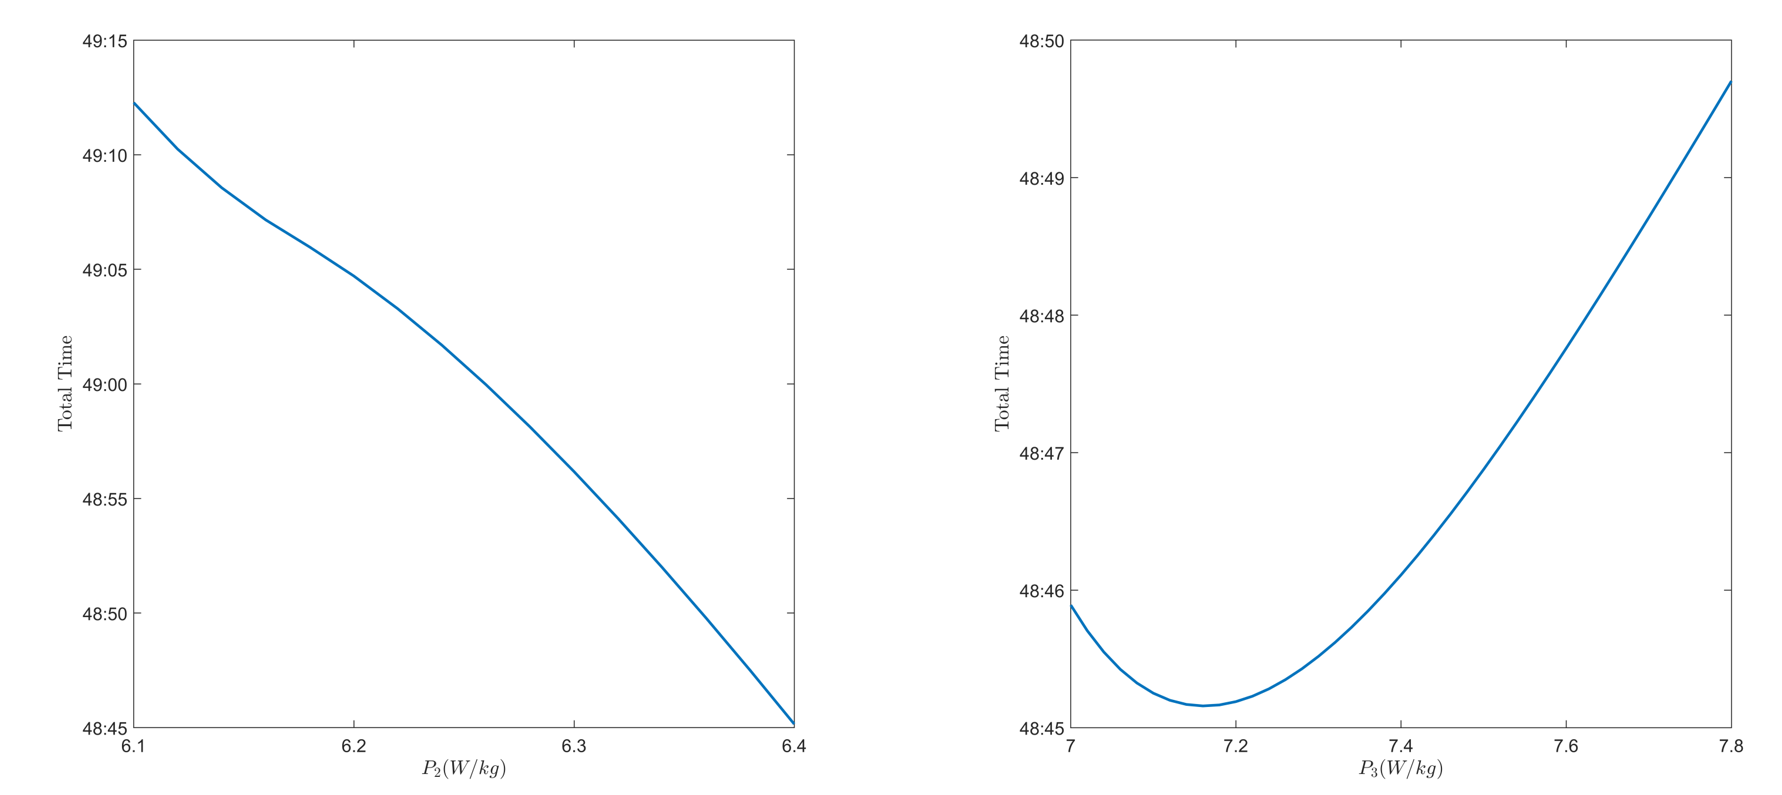
\includegraphics[width=0.7\linewidth]{image/p1}
	\caption{MTT Model sensitivity regarding $P_2$ and $P_3$}
	\label{P1}
\end{figure}
\par Through the same method, we obtain multiple sets of data and plotted the function between power output of two stages and total time for MTT [\ref{P1}]. 
\par As is shown in the curve, change in total time is always smaller as the output power changes at different stages, which shows that though riders does not have precise control over speed and power output, their score won't be much worse if follow our strategy. Also, the same method can be applied to the female virtual rider by changing the constraints and figuring out the optimal tactic, shown in table [\ref{time3}].
\begin{table}[h]
	%		\renewcommand\arraystretch{0.9}
	\setlength\tabcolsep{13pt}%调列距
	\setlength{\belowcaptionskip}{0.2cm}
	\centering
	\caption{Strategies under different constraints for female}
	\begin{tabular}{ccc|cccc}
		\toprule[2pt]
		$P_1$    & $P_2$    & $P_3$    & $T_1$    & $T_2$    & $T_3$    & Total Time \\
		\midrule
FTP   & 5.61  & 6.50  & 28:01 & 3:17  & 7:08  & 38:28 \\
FTP   & \textbf{5.50 } & 6.34  & 25:20 & 4:22  & 8:49  & 38:32 \\
FTP   & \textbf{5.40 } & 6.34  & 23:57 & 5:53  & 8:49  & 38:40 \\
FTP   & 5.61  & \textbf{6.60 } & 28:52 & 3:17  & 6:19  & 38:29 \\
FTP   & 5.61  & \textbf{6.70 } & 29:34 & 3:17  & 5:38  & 38:30 \\
	\bottomrule[2pt]
\end{tabular}%
\label{time3}%
\end{table}%
% TODO: \usepackage{graphicx} required
\begin{figure}[h]
	\centering
	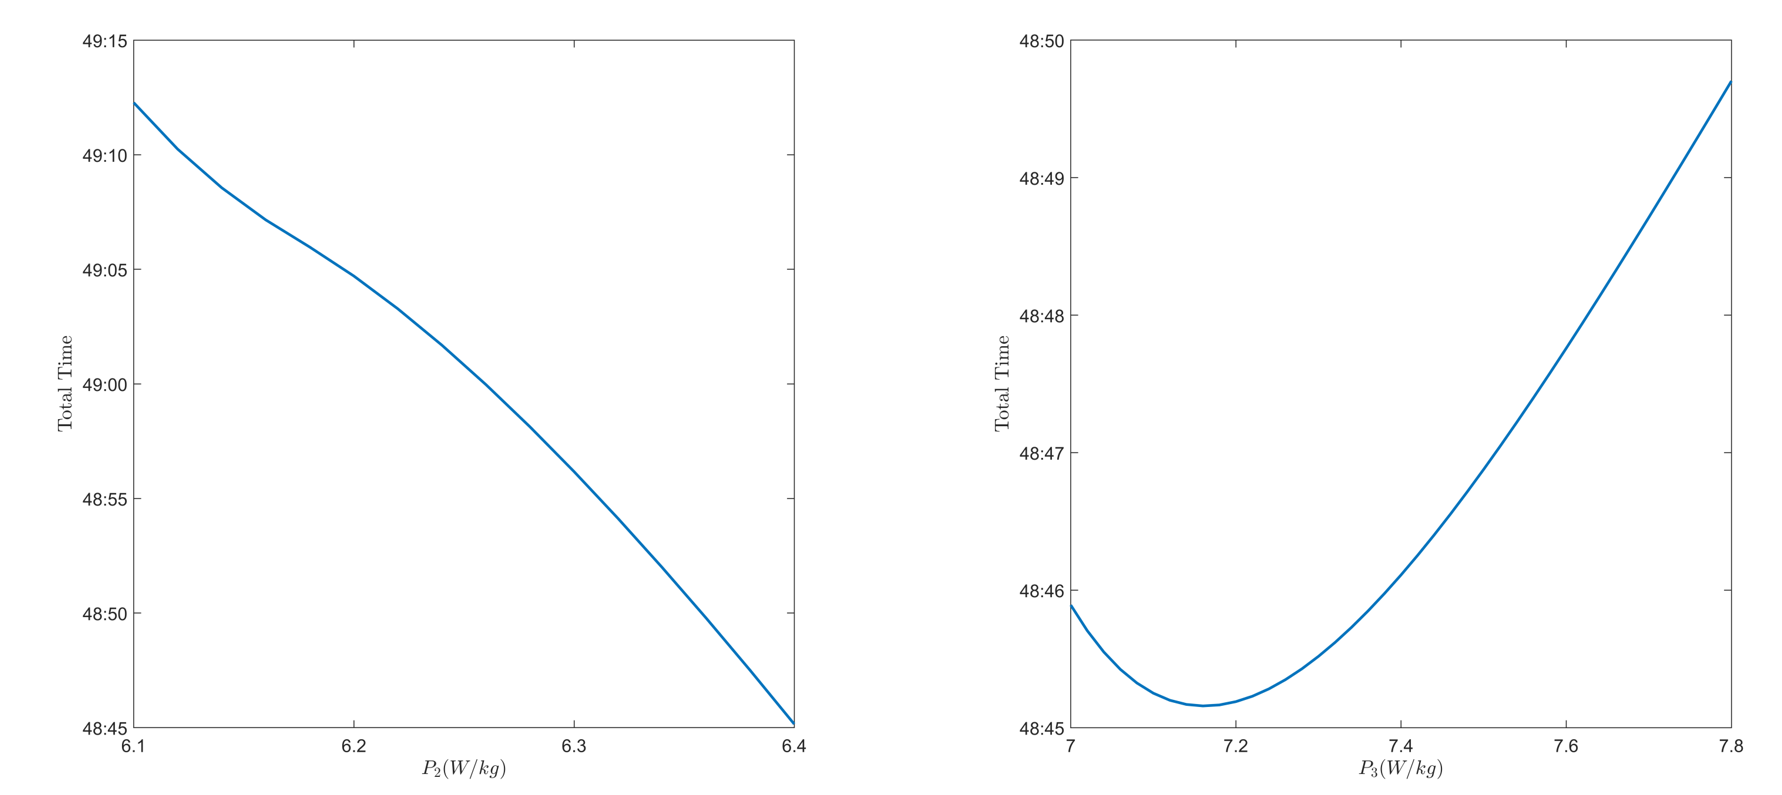
\includegraphics[width=0.7\linewidth]{image/p1}
	\caption{FTT Model sensitivity regarding $P_2$ and $P_3$}
	\label{P2}
\end{figure}

\par It can be inferred from the table that minor changes in power output won't cause significant difference in final scores(Total Time).Through the same method, multiple sets of data can be obtained by changing constraints, and the function is plotted between power output of two stages and total time  for FTT[\ref{P2}]. 
\par In conclusion, although our model can vary with output power, the change in total time is continuous with respect to the change in output power. Also, the change in total time is not significant with respect to variation in power output in different stages. As a result, it can be concluded that athletes can achieve ideal results within a power output range.


\section{Model Extension and Evaluation}
\subsection{Extension for team time trial}
\par Team time trial (TTT) is generally composed of six drivers as a team, and the fourth-place finisher in the team will be the team result. Teams generally use a straight-line formation, with a gap of 30-50 cm between riders, so that the rider at the front can block the wind for others behind. When the team is moving at a constant speed, the required output power per kilogram decreases from the head of the row to the end [\ref{beauty}], as does the energy per kilogram required to complete a unit of distance.
% TODO: \usepackage{graphicx} required
\begin{figure}[h]
	\centering
	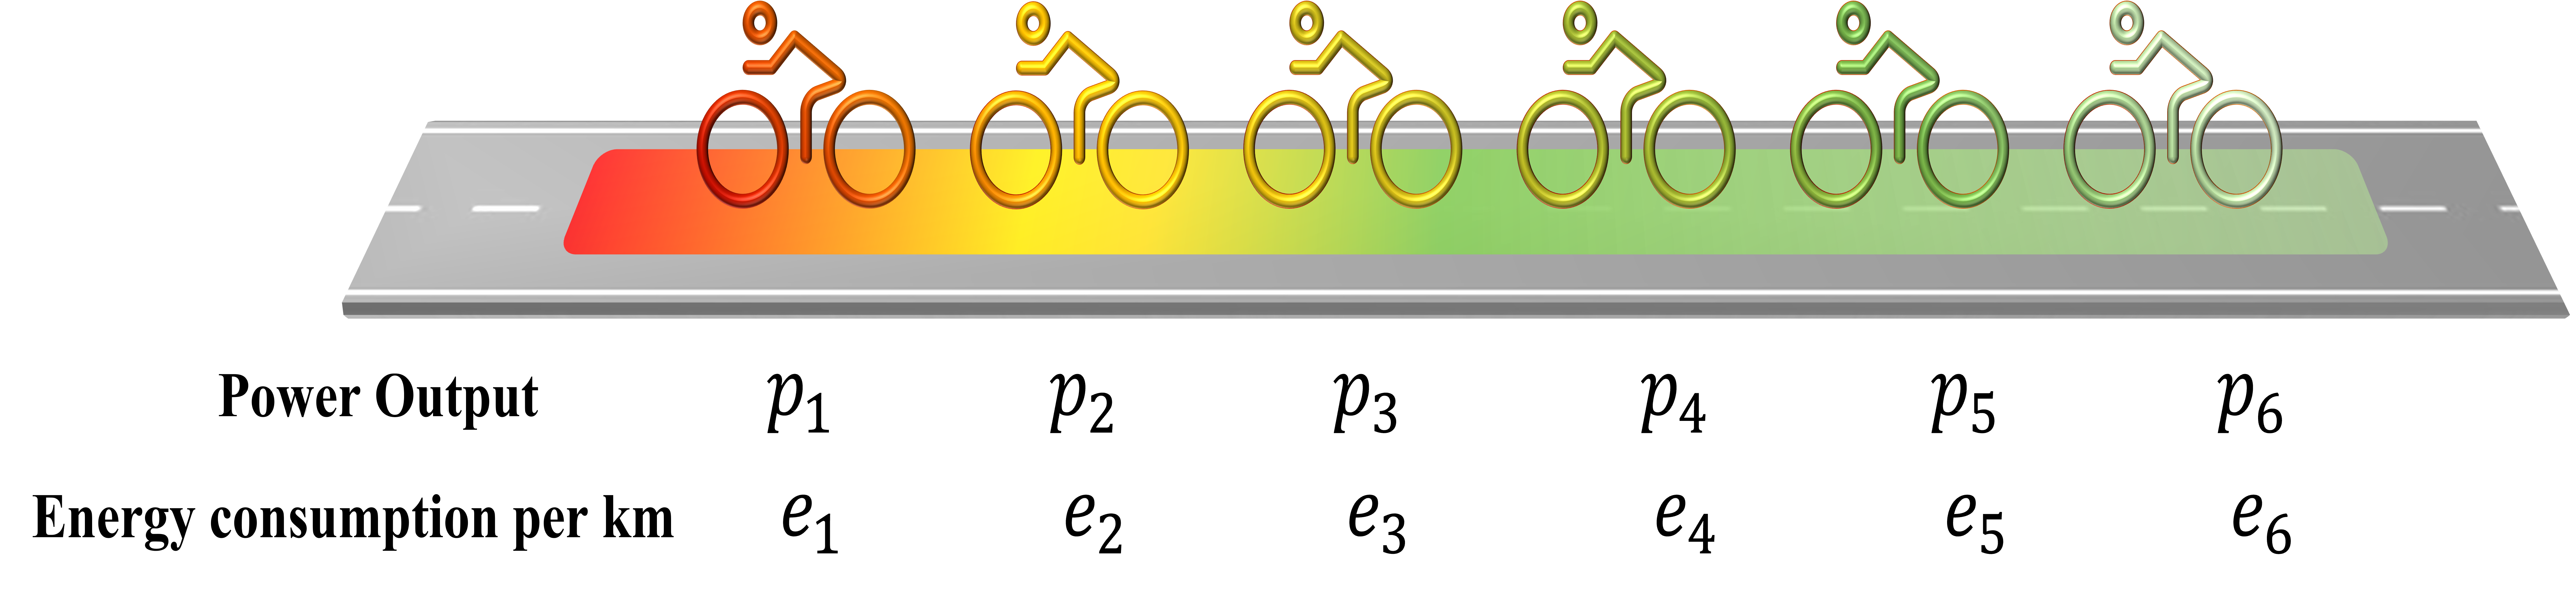
\includegraphics[width=1\linewidth]{image/beauty}
	\caption{Team time trialist diagram}
	\label{beauty}
\end{figure}

\par After watching some races, we find that teams generally have only four riders when they are approaching the finish line, leaving the remaining two far behind due to lack of energy. When we extend the model to team time trial, the six drivers shall be split into a stronger four and a weaker two, which will fall behind in the race.

\par In our model extension, riders in the team take turns taking the lead to block the wind and move forward at a constant speed $\nu$. The entire race process is divided into three stages, with 6, 5, and 4 riders making up the team respectively, and each stage consists of several same leading cycles. A leading period refers to the period from when a rider leaves the lead position to the next lead.

\par Let $\sigma_j(j\leq3)$ be the track of stage $j$, $p_i(i\leq6)$ be the power output per kilogram of the $i^{th}$ position in formation, and $e_i(s)(i\leq6)$ be the cost of energy per kilogram to complete 1 km. Moreover, $N_j$ is used to denote the number of leading cycles with length $T_j$ included in stage $j$.

\par This way, we can list the corresponding PTE equations for each stage: 

\begin{equation}\label{PTEeqs}
	\begin{split}
		\left\{
	\begin{aligned}
	N_1p_1T_1 &=\sum_{i=1}^{6}\int_{\sigma_1}e_i(s)ds  \\
	N_2p_2T_2 &=\sum_{i=1}^{5}\int_{\sigma_2}e_i(s)ds  \\
	N_3p_3T_3 &=\sum_{i=1}^{4}\int_{\sigma_3}e_i(s)ds  
	\end{aligned}
	\right.
\end{split}
\end{equation}

\par and the following constraints:

\begin{equation}\label{teamcons}
\begin{split}
		\left\{
		\begin{aligned}
	&(N_1-1)T_1<f_6^{-1}(p_6)\leq N_1T_1 \\
	&(N_2-1)T_2<f_5^{-1}(p_5)+N_1T_1\leq N_2T_2 \\
	&N_3T_3 \leq f_4^{-1}(p_4)
\end{aligned}
\right.
\end{split}
\end{equation}

\par where $f_i$ is the power curve of $i^{th}$ most energetic and powerful rider in the team.

\par Constraints (\ref{teamcons}) point out when the two weakest players in the team will be exhausted and fall behind. And we can give the best strategy for the team by solving an optimization problem similar to (\ref{min})(\ref{cons3})  in our PTE model:

\begin{equation}
	\min N_1T_1+N_2T_2+N_3T_3 \quad\quad \rm{s.t.}
\end{equation}

\begin{equation}
\begin{split}
	\left\{
	\begin{aligned}
	&N_jp_jT_j =\sum_{i=1}^{7-j}\int_{\sigma_j}e_i(s)ds,j=1,2,3\\
	&(N_1-1)T_1<f_6^{-1}(p_6)\leq N_1T_1 \\
	&(N_2-1)T_2<f_5^{-1}(p_5)+N_1T_1\leq N_2T_2 \\
	&N_3T_3 \leq f_4^{-1}(p_4)
\end{aligned}
		\right.
\end{split}
\end{equation}

\par Of course, PTE model for TTT can take into account more factors, such as considering the movement of the team as a speed change motion, and considering environmental factors such as weather and slope, so as to induce the expression of $e_i(s)$. At the same time, we can also establish the relationship between $p_i$ and $e_i$ through the speed $\nu$. Although these works require more computational resources and data, they can all be refined within the framework of our PTE model.

\subsection{Strengths}

\begin{itemize}
	\item {\bf } Four optimization methods are applied to find optimal power distribution during cycling in the second question and they converge to same results, which ensures robustness of our model.

	\item {\bf } In the application, we compare results from virtual time trialists with Olympics racers and real-life riders which verifies the reliability and rationality of model in the second and third question.

	\item {\bf } To characterize the effect of wind direction in the model, we propose and prove a theorem based on mathematical principles, which lays the scientific foundation of sensitivity analysis in the third question.

	\item {\bf } PTE Model can be extended naturally to a variety of cycling competitions, both individual and team, which reflects broad applicability of Our model.
\end{itemize}

\subsection{Weaknesses}

\begin{itemize}
	\item {\bf } The analysis of rider's power profile and tactics based on our model can be more accurate if we have sufficient complete data about different kinds of riders' power output.
\end{itemize}

\begin{itemize}
	\item {\bf } Our model can be easily applied to tracks within half an hour to an hour of riding. However, for courses like Tour de France, our model has not been tested enough.
\end{itemize}
\begin{thebibliography}{99}

\bibitem{1} Leo, P., Spragg, J., Podlogar, T. et al. Power profiling and the power-duration relationship in cycling: a narrative review. Eur J Appl Physiol 122, 301–316 (2022).
\bibitem{2} Sanders, D., van Erp, T., $\&$ de Koning, J. J. (n.d. ). Intensity and Load Characteristics of Professional Road Cycling: Differences Between Men’s and Women’s Races, International Journal of Sports Physiology and Performance, 14(3), 296-302.
\bibitem{3} Rudin W. Principles of mathematical analysis[M]. New York: McGraw-hill, 1976.
\bibitem{4} Van Erp T, Sanders D, De Koning J J. Training characteristics of male and female professional road cyclists: a 4-year retrospective analysis[J]. International journal of sports physiology and performance, 2019, 15(4): 534-540.
\bibitem{5} Van Erp T, Lamberts RP, Sanders D. Power Profile of Top 5 Results in World Tour Cycling Races. Int J Sports Physiol Perform. 2022 Feb 1;17(2):203–209.





\end{thebibliography}
\newpage
\begin{appendices}
	
	\section{MATLAB Code for Power Curve Fitting}
	
	\textbf{\textcolor[rgb]{0.98,0.00,0.00}{fitting.m}}
	\lstinputlisting[language=Matlab]{./code/fitting.m}
	
	\section{MATLAB Code for Optimization}
	
 \textcolor[rgb]{0.98,0.00,0.00}{\textbf{Optimization.m}}
	\lstinputlisting[language=Matlab]{./code/Optimization.m}
	 \textcolor[rgb]{0.98,0.00,0.00}{\textbf{fun.m}}
	\lstinputlisting[language=Matlab]{./code/fun.m}
		 \textcolor[rgb]{0.98,0.00,0.00}{\textbf{nonlfun.m}}
	\lstinputlisting[language=Matlab]{./code/nonlfun.m}
			 \textcolor[rgb]{0.98,0.00,0.00}{\textbf{finv.m}}
	\lstinputlisting[language=Matlab]{./code/finv.m}
\end{appendices}



\end{document}
